\documentclass{article} 
\usepackage[T1]{fontenc}
\usepackage{fontspec} % Gói hỗ trợ font chữ, chống lỗi missing character
\usepackage[utf8]{inputenc}
\usepackage[vietnamese]{babel}
\usepackage{graphicx} % Required for inserting images
\usepackage{amsmath}
\usepackage{geometry}
\usepackage{pifont}
\usepackage{hyperref}
\usepackage{tocloft}
\usepackage{longtable}
\usepackage{float} 
\usepackage{forest}
\usepackage{array}
\usepackage{ragged2e}
\usepackage{enumerate}
\usepackage{caption}
\usepackage{tcolorbox}
\usepackage{titlesec}
\usepackage{fancyhdr} % Gói tạo header/footer
\usepackage{tikz} % Goi ve hinh

\renewcommand{\arraystretch}{1.2} % Điều chỉnh chiều cao hàng

\setcounter{tocdepth}{4}
\setcounter{secnumdepth}{4}

\usetikzlibrary{shapes.geometric, arrows}

% Define styles for blocks
\tikzstyle{startstop} = [rectangle, rounded corners, minimum width=3cm, minimum height=1cm,text centered, draw=black, fill=red!30]
\tikzstyle{process} = [rectangle, minimum width=3cm, minimum height=1cm, text centered, draw=black, fill=blue!30]
\tikzstyle{decision} = [diamond, minimum width=3cm, minimum height=1cm, text centered, draw=black, fill=green!30]
\tikzstyle{arrow} = [thick,->,>=stealth]

% =================== Changing font ========================
% \usepackage{cmbright}

% \usepackage{tgheros}
% \renewcommand{\familydefault}{\sfdefault} % Chọn sans-serif làm mặc định

\usepackage{lmodern}
\renewcommand{\familydefault}{\sfdefault} % Chuyển toàn bộ tài liệu sang sans-serif

% \usepackage{mathpazo}
%=========================================================

% Cài đặt kích thước trang
\geometry{top=2cm, bottom=2.5cm, left=3.0cm, right=3.0cm}

% Tùy chỉnh màu sắc liên kết (tùy chọn)
\hypersetup{
    colorlinks=true,
    linkcolor=blue, % Đặt màu liên kết là màu xanh
    citecolor=black, % Màu liên kết trích dẫn
    filecolor=black,
    urlcolor=blue,
    pdftitle={Chủ đề 2},
    pdfpagemode=FullScreen,
}

% ================= Header & Footer ======================
% Tạo lệnh Header & Footer
\pagestyle{empty}  % Mặc định là không có header và footer
\newcommand{\setheadersfooters}{
    \pagestyle{fancy}
    % Header
    \lhead{EM1180 - 158853}
    \chead{}
    \rhead{GVHD: TS. Nguyễn Thị Thanh Dần}
    % Footer
    \lfoot{Nhóm 3}
    \cfoot{\thepage}
    \rfoot{\today}
}
% ========================================================

% ==================================== Trang bìa ======================================
\title{
    \begin{center}
        \fontsize{16}{16}\selectfont \textbf{ĐẠI HỌC BÁCH KHOA HÀ NỘI} \\[0.1cm]
        \fontsize{14}{14}\selectfont \textnormal{TRƯỜNG KINH TẾ}
    \end{center}
    \vspace{2em} 
    \begin{center}
        
\includegraphics[width=6cm]{logo.jpg} 
    \end{center}
    \vspace{1em} 
    \begin{center}
        \fontsize{16}{16}\selectfont \textbf{BÁO CÁO BÀI TẬP LỚN} \\[1em]
        \fontsize{16}{16}\selectfont \textbf{VĂN HÓA KINH DOANH VÀ TINH THẦN KHỞI NGHIỆP} \\[1em]
        \fontsize{14}{16}\selectfont CHỦ ĐỀ 2: TRÌNH BÀY VỀ ĐẠO ĐỨC KINH DOANH HOẶC TRÁCH NHIỆM XÃ HỘI CỦA MỘT DOANH NGHIỆP CỤ THỂ (Coca-Cola)
    \end{center}
}

\author{
    \textbf{Giảng viên hướng dẫn} \\[0.5em]
    \textnormal{TS Nguyễn Thị Thanh Dần} \\[2em]
    \textbf{Nhóm 3 - Lớp 158853} \\[0.5em]
    \begin{tabular}{l l}
        Đỗ Gia Huy          & 20215060 \\
        Bùi Minh Tiến   & 20232324 \\
        Dương Thị Huyền Trang         & 20223323 \\
        Phan Đoàn Minh Nghĩa    & 20230470 \\
        Nguyễn Minh Quân        & 20225520 \\
    \end{tabular}
} 

\date { \vspace{2em} Hà Nội, \today}
 
\begin{document}

\maketitle
\thispagestyle{empty}

\newpage
\tableofcontents

\newpage
\setheadersfooters

\vspace{5cm}

\begin{table}[H]
\centering
\textbf{\Large Bảng phân công nhiệm vụ} \\[1em]
\begin{tabular}{|p{4cm}|p{8cm}|>{\centering\arraybackslash}p{2cm}|}
\hline
\textbf{Tên thành viên} & \textbf{Nhiệm vụ}               & \textbf{\% Đóng góp} \\ \hline
Đỗ Gia Huy              & Tổng hợp \& viết báo cáo        & 20\%                 \\ \hline
Dương Thị Huyền Trang   & Mục 1 \& 2 phần 1               & 20\%                 \\ \hline
Phan Đoàn Minh Nghĩa    & Mục 3 \& 4 phần 1               & 20\%                 \\ \hline
Bùi Minh Tiến           & Mục 1 \& 2 phần 2               & 20\%                 \\ \hline
Nguyễn Minh Quân        & Mục 3 \& 4 phần 2 \& phần 3     & 20\%                 \\ \hline
\end{tabular}
\label{tab:tasks}
\end{table}

\newpage

% ==================================  Lời nói đầu ====================================
\section*{Lời nói đầu}
Đạo đức kinh doanh là một trong những vấn đề cốt lõi và có ảnh hưởng sâu rộng nhất trong môi trường kinh doanh hiện đại. Tuy nhiên, đây cũng là khái niệm dễ bị hiểu sai, diễn giải mơ hồ hoặc bị lợi dụng để che đậy những mục tiêu không minh bạch. Trong hơn hai thập kỷ qua, đạo đức kinh doanh đã nổi lên như một chủ đề được quan tâm rộng rãi, không chỉ bởi các nhà làm chính sách và các học giả, mà còn bởi chính các doanh nghiệp và người tiêu dùng. Áp lực xã hội ngày càng gia tăng đã buộc các doanh nghiệp phải cân nhắc nhiều hơn đến tác động đạo đức trong từng quyết định quản trị, từ chiến lược sản phẩm, quảng cáo, tuyển dụng, đến hoạt động đầu tư và môi trường. Người tiêu dùng ngày nay không chỉ quan tâm đến chất lượng sản phẩm hay giá cả, mà còn đánh giá doanh nghiệp dựa trên thái độ đối với môi trường, quyền lợi người lao động, tính minh bạch trong tài chính và trách nhiệm xã hội nói chung. Đồng thời, các cơ quan lập pháp cũng đã ban hành nhiều quy định nhằm khuyến khích và bắt buộc doanh nghiệp hành xử một cách có trách nhiệm, văn minh và nhân bản hơn.

\vspace{0.5cm}
Hoạt động kinh doanh không diễn ra trong khoảng không trống rỗng, mà luôn tác động trực tiếp đến mọi mặt của đời sống kinh tế, xã hội và môi trường. Vì vậy, mỗi nhà kinh doanh cần ý thức được vai trò đạo đức nghề nghiệp trong hành vi và quyết định của mình. Kinh doanh không thể tách rời khỏi khuôn khổ pháp luật; một doanh nghiệp chỉ có thể phát triển bền vững khi tuân thủ những giới hạn mà xã hội đặt ra thông qua luật pháp và chuẩn mực đạo đức chung. Nếu vượt ra khỏi những giới hạn này, không chỉ rủi ro pháp lý mà còn là nguy cơ đánh mất niềm tin của công chúng — một tài sản vô hình nhưng vô cùng quý giá. Phẩm chất đạo đức của người làm kinh doanh chính là nền móng tạo nên uy tín cá nhân và thương hiệu doanh nghiệp, giúp doanh nghiệp đứng vững trước sóng gió cạnh tranh, thu hút được nhân tài, giữ chân khách hàng và từ đó đạt được sự thành công dài hạn. Sự phát triển bền vững của một doanh nghiệp không chỉ dựa vào năng lực tài chính hay công nghệ, mà còn phụ thuộc rất lớn vào mức độ gắn kết giữa các mục tiêu kinh tế với những cam kết đạo đức rõ ràng. Chính vì vậy, trong thời đại toàn cầu hóa và hội nhập sâu rộng hiện nay, đạo đức kinh doanh không còn là lựa chọn, mà đã trở thành điều kiện tiên quyết cho sự tồn tại và thành công bền vững của bất kỳ doanh nghiệp nào.
\vspace{1cm}

% ========================= Phần 1 ==========================
\newpage
\section{Cơ sở lý thuyết về đạo đức kinh doanh và trách nhiệm xã hội của một doanh nghiệp}
\subsection{Khái niệm, vai trò}
    \subsubsection{Đạo đức kinh doanh}
        \paragraph{Khái niệm đạo đức kinh doanh}
            \vspace{0.2cm}
            Đạo đức kinh doanh là một tập hợp các nguyên tắc, chuẩn mực có tác dụng điều chỉnh, đánh giá, hướng dẫn và kiểm soát hành vi của các chủ thể kinh doanh.Chúng được những người hữu quan (như người đầu tư, khách hàng, người quản lý, người lao động, đại diện cơ quan pháp lý, cộng đồng dân cư, đối tác, đối thủ,...) sử dụng để phán xét một hành động cụ thể là đúng hay sai, hợp đạo đức hay phi đạo đức.
            
            \vspace{0.2cm}
            Đạo đức kinh doanh chính là đạo đức được vận dụng vào trong hoạt động kinh doanh, tạo cơ sở để các doanh nhân lựa chọn phương thức kinh doanh
            
            \vspace{0.2cm}
            Đạo đức kinh doanh là một dạng đạo đức nghề nghiệp: Đạo đức kinh doanh có tính đặc thù của hoạt động kinh doanh, do kinh doanh là hoạt động gắn liền với các lợi ích kinh tế, do vậy khía cạnh thể hiện trong ứng xử về đạo đức không hoàn toàn giống các hoạt động khác: Tính thực dụng, sự coi trọng hiệu quả kinh tế là những đức tính tốt của giới kinh doanh nhưng nếu áp dụng sang các lĩnh vực khác như giáo dục, y tế... hoặc sang các quan hệ xã hội khác như vợ chồng, cha mẹ, con cái thì đó lại là những thói xấu bị xã hội phê phán. Song cần lưu ý rằng đạo đức kinh doanh vẫn luôn phải chịu sự chi phối bởi một hệ giá trị và chuẩn mực đạo đức xã hội chung.

        \paragraph{Vai trò của đạo đức kinh doanh}
            \vspace{0.2cm}
            Lợi nhuận là một trong những yếu tố cần thiết cho sự tồn tại của một doanh nghiệp và là cơ sở đánh giá khả năng duy trì hoạt động kinh doanh của doanh nghiệp. Tuy nhiên, nếu người quản lý doanh nghiệp hiểu sai bản chất của lợi nhuận và coi đấy là mục tiêu chính và duy nhất của hoạt động kinh doanh thì sự tồn tại của doanh nghiệp có thể bị đe doạ. Tẩm quan trọng của đạo đức kinh doanh đối với một tổ chức là một vấn đề gây tranh cãi với rất nhiều quan điểm khác nhau. Nhiều giám đốc doanh nghiệp coi các chương trình đạo đức là một hoạt động xa xỉ, chỉ mang lại lợi ích cho xã hội chứ không phải doanh nghiệp. Vai trò của sự quan tâm đến đạo đức trong các mối quan hệ kinh doanh tiếp tục bị hiểu lầm. Chúng ta sẽ xem xét ở các nội dung dưới đây về vai trò của đạo đức kinh doanh trong hoạt động quản trị doanh nghiệp.

            \begin{figure}[H]
                \centering
                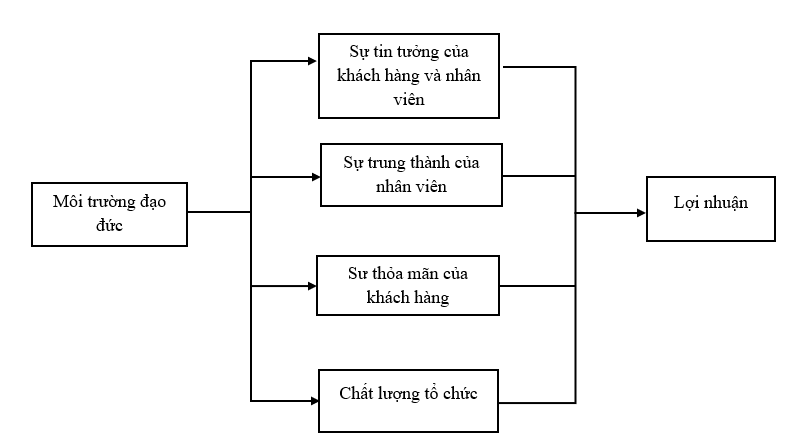
\includegraphics[width=0.8\textwidth]{assert/img1.png}
                \caption{Vai trò của đạo đức tổ chức trong hoạt động kinh doanh}
                \label{fig:img1}
            \end{figure}

            \begin{itemize}
                \item \textbf{Đạo đức trong kinh doanh góp phần điều chỉnh hành vi của các chủ thể kinh doanh:}

                \qquad Đạo đức kinh doanh bổ sung và kết hợp với pháp luật điều chỉnh các hành vi kinh doanh theo khuôn khổ pháp luật và quỹ đạo của các chuẩn mực đạo đức xã hội. Không một pháp luật nào, dù hoàn thiện đến đâu chăng nữa cũng có thể là chuẩn mực cho mọi hành vi của đạo đức kinh doanh. Nó không thể thay thế vai trò của đạo đức kinh doanh trong việc khuyến khích mọi người làm việc thiện, tác động vào lương tâm của doanh nhân. Bởi vì phạm vi ảnh hưởng của đạo đức rộng hơn pháp luật, nó bao quát mọi lĩnh vực của thế giới tinh thần, trong khi pháp luật chỉ điều chỉnh những hành vi liên quan đến chế độ nhà nước, chế độ xã hội... Mặt khác, pháp luật càng đẩy đủ, chặt chẽ và được thi hành nghiêm chỉnh thì đạo đức càng được đề cao, càng hạn chế được sự kiếm lời phi pháp. Tham nhũng, buôn lậu, trốn thuế, gian lận thương mại... khi bị phát hiện sẽ bị pháp luật điều chỉnh, lúc này “hiện tượng kiện tụng buộc người ta phải cư xử có đạo đức".

                \qquad Các mức độ bổ sung, "dung hòa” đạo đức và pháp luật được khái quát qua các “góc vuông xác định tính chất đạo đức và pháp lý của hành vi".

                \qquad Sự tồn vong của doanh nghiệp không chỉ do chất lượng của bản thân các sản phẩm, dịch vụ cung ứng mà còn chủ yếu do phong cách kinh doanh của doanh nghiệp. Hành vi kinh doanh thể hiện tư cách của doanh nghiệp, và chính tư cách ấy tác động trực tiếp đến sự thành bại của tổ chức. Đạo đức kinh doanh, trong chiều hướng ấy, trở thành một nhân tố chiến lược trong việc phát triển doanh nghiệp. Chẳng phải vô cớ mà khoảng 15 năm nay một ngạn ngữ Ấn Độ được lưu truyền trong giới doanh nghiệp ở các nước phát triển: "gieo tư tưởng gặt hành vi, gieo hành vi gặt thói quen, gieo thói quen gặt tư cách, gieo tư cách gặt số phận".

                \item \textbf{Đạo đức kinh doanh góp phần vào chất lượng của doanh nghiệp:}
                
                \qquad Phần thưởng cho một công ty có quan tâm đến đạo đức là được các nhân viên, khách hàng và công luận công nhận là có đạo đức. Phần thưởng cho trách nhiệm đạo đức và trách nhiệm xã hội trong các quyết định kinh doanh bao gồm hiệu quả trong các hoạt động hàng ngày tăng cao, sự tận tâm của các nhân viên, chất lượng sản phẩm được cải thiện, đưa ra quyết định đúng đắn hơn, sự trung thành của khách hàng và lợi ích về kinh tế lớn hơn. Các tổ chức phát triển được một môi trường trung thực và công bằng sẽ gây dựng được nguồn lực đáng quý có thể mở rộng cánh cửa dẫn đến thành công.

                \qquad Các tổ chức được xem là có đạo đức thường có nền tảng là các khách hàng trung thành cũng như đội ngũ nhân viên vững mạnh, bởi sự tin tưởng và phụ thuộc lẫn nhau trong mối quan hệ. Nếu các nhân viên hài lòng thì khách hàng sẽ hài lòng và nếu khách hàng hài lòng thì các nhà đầu tư sẽ hài lòng. Các khách hàng có xu hướng thích mua hàng của các công ty liêm chính hơn, đặc biệt là khi giá cả của công ty đó cũng bằng với giá của các công ty đối thủ. Khi các nhân viên cho rằng tổ chức của mình có một môi trường đạo đức, họ sẽ tận tâm hơn và hài lòng với công việc của mình hơn. Các công ty cung ứng thường muốn làm ăn lâu dài với các công ty mà họ tin tưởng để qua hợp tác họ có thể xoá bỏ được sự không hiệu quả, các chi phí và những nguy cơ để có thể làm hài lòng khách hàng. Các nhà đầu tư cũng rất quan tâm đến vấn để đạo đức, trách nhiệm xã hội và uy tín của các công ty mà họ đầu tư, và các công ty quản lý tài sản có thể giúp các nhà đầu tư mua cổ phiếu của các công ty có đạo đức. Các nhà đầu tư nhận ra rằng, một môi trường đạo đức là nền tảng cho sự hiệu quả, năng suất, và lợi nhuận. Mặt khác, các nhà đầu tư cũng biết rằng các hình phạt hay công luận tiêu cực cũng có thể làm giảm giá cổ phiếu, giảm sự trung thành của khách hàng và đe doạ hình ảnh lâu dài của công ty. Các vấn để về pháp lý và công luận tiêu cực có những tác động rất xấu tới sự thành công của bất cứ một công ty nào.

                \qquad Sự lãnh đạo cũng có thể mang lại các giá trị tổ chức và mạng lưới xã hội ủng hộ các hành vi đạo đức. Các nhà lãnh đạo nhận thức được bản chất của mối quan hệ trong kinh doanh, những vấn để và mâu thuẫn tiềm ẩn, tìm ra biện pháp quản lý khắc phục những trở ngại có thể dẫn đến bất đồng, tạo dựng bầu không khí làm việc thuận lợi cho mọi người hòa đồng, tìm ra được một hướng chung tạo ra sức mạnh tổng hợp của sự đồng thuận, đóng góp cho sự phát triển của tổ chức. Sự lãnh đạo chú trọng vào việc xây dựng các giá trị đạo đức tổ chức vững mạnh cho các nhân viên sẽ tạo ra sự đồng thuận về chuẩn tắc đạo đức và đặc điểm của những mối quan hệ chung. Các lãnh đạo ở địa vị cao trong tổ chức đóng một vai trò chủ chốt trong việc truyền bá các tiêu chuẩn đạo đức, các chuẩn tắc và quy định đạo đức nghề nghiệp. Sự cần thiết có sự lãnh đạo có đạo đức để cung cấp cơ cấu cho các giá trị của tổ chức và những ngăn cản đối với các hành vi vô đạo đức đã được làm rõ trong nghiên cứu trước. Các nhà lãnh đạo có thể cung cấp cơ cấu này bằng cách thiết lập các chương trình đào tạo đạo đức chính thức và không chính thức, cũng như các hướng dẫn khác, giúp các nhân viên phải lưu tâm đến khía cạnh đạo đức trong quá trình đưa ra quyết định của mình.

                \qquad Nhận thức của các nhân viên về công ty của mình là có một môi trường đạo đức sẽ mang lại những kết quả tốt đẹp trong hoạt động của tổ chức. Xét về khía cạnh năng suất và làm việc theo nhóm, các nhân viên trong các phòng ban khác nhau cũng như giữa các phòng ban cần thiết có chung một cái nhìn về sự tin tưởng. Mức độ tin tưởng cao hơn có ảnh hưởng lớn nhất lên các mối quan hệ trong nội bộ các phòng ban hay các nhóm làm việc, nhưng tin tưởng cũng là một nhân tố quan trọng trong các mối quan hệ giữa các phòng ban trong tổ chức. Bởi vậy, các chương trình tạo ra một môi trường lao động có lòng tin sẽ làm cho các nhân viên sẵn sàng hành động theo các quyết định và hành động của các đồng nghiệp. Trong một môi trường làm việc như thế này, các nhân viên có thể mong muốn được các đồng nghiệp và cấp trên đối xử với mình với một sự tôn trọng và quan tâm sâu sắc. Các mối quan hệ có lòng tin trong một tổ chức giữa các giám đốc và cấp dưới của họ và ban quản lí cấp cao góp phần vào hiệu quả của quá trình đưa quyết định.

                \qquad Hầu hết các công ty đáng ngưỡng mộ nhất trên thế giới đều chú trọng vào phương pháp làm việc theo nhóm, quan tâm nhiều đến khách hàng, đề cao việc đối xử công bằng với nhân viên, và thưởng cho các thành tích tốt.

                \item \textbf{Đạo đức kinh doanh góp phần vào sự cam kết và tận tâm của nhân viên:}
                
                \qquad Sự tận tâm của nhân viên xuất phát từ việc các nhân viên tin rằng tương lai của họ gắn liền với tương lai của doanh nghiệp và chính vì thế họ sẵn sàng hy sinh cá nhân vì tổ chức của mình. Doanh nghiệp càng quan tâm đến nhân viên bao nhiêu thì các nhân viên càng tận tâm với doanh nghiệp bấy nhiêu. Các vấn đề có ảnh hưởng đến sự phát triển của một môi trường đạo đức cho nhân viên bao gồm một môi trường lao động an toàn, thù lao thích đáng, và thực hiện đầy đủ các trách nhiệm được ghi trong hợp đồng với tất cả các nhân viên. Các chương trình cải thiện môi trường đạo đức có thể là chương trình "gia đình và công việc" hoặc chia/bán cổ phần cho nhân viên. Các hoạt động từ thiện hoặc trợ giúp cộng đồng không chỉ tạo ra suy nghĩ tích cực của chính nhân viên về bản thân họ và doanh nghiệp mà còn tạo ra sự trung thành của nhân viên đối với doanh nghiệp.

                \qquad Sự cam kết làm các điều thiện và tôn trọng nhân viên thường tăng sự trung thành của nhân viên đối với tổ chức và sự ủng hộ của họ với các mục tiêu của tổ chức. Các nhân viên sẽ dành hầu hết thời gian của họ tại nơi làm việc chứ không chây ì, “chỉ làm cho xong công việc mà không có nhiệt huyết" hoặc làm việc “qua ngày đoạn tháng", không tận tâm đối với những mục tiêu đề ra của tổ chức bởi vì họ cảm thấy mình không được đối xử công bằng.

                \qquad Môi trường đạo đức của tổ chức rất quan trọng đối với các nhân viên. Đa số nhân viên tin rằng, hình ảnh của một công ty đối với cộng đồng là vô cùng quan trọng, các nhân viên thấy công ty của mình tham gia tích cực vào các công tác cộng đồng sẽ cảm thấy trung thành hơn với cấp trên và cảm thấy tích cực về bản thân họ. Khi các nhân viên cảm thấy môi trường đạo đức trong tổ chức có tiến bộ, họ sẽ tận tâm hơn để đạt được các tiêu chuẩn đạo đức cao trong các hoạt động hàng ngày. Các nhân viên sẵn lòng thảo luận các vấn để đạo đức và ủng hộ các ý kiến nâng cao chất lượng trong công ty nếu công ty đó cam kết sẽ thực hiện các quy định đạo đức. Thực chất, những người được làm việc trong một môi trường đạo đức tin rằng họ sẽ phải tôn trọng tất cả các đối tác kinh doanh của mình, không kể những đối tác ấy ở bên trong hay bên ngoài công ty. Họ cần phải cung cấp những giá trị tốt nhất có thể cho tất cả các khách hàng và các cố đông.

                \qquad Cam kết của nhân viên đối với chất lượng của công ty có tác động tích cực đến vị thế cạnh tranh của công ty nên một môi trường làm việc có đạo đức có tác dụng tích cực đến các điểm mấu chốt về tài chính. Bởi chất lượng những dịch vụ phục vụ khách hàng tác động đến sự hài lòng của khách hàng, nên những cải thiện trong các dịch vụ phục vụ khách cũng sẽ có tác động trực tiếp lên hình ảnh của công ty, cũng như khả năng thu hút các khách hàng mới của công ty.

                \item \textbf{Đạo đức kinh doanh góp phần làm hài lòng khách hàng:}
                
                \qquad Các nghiên cứu và kinh nghiệm hiện thời của nhiều quốc gia cho thấy mối quan hệ chặt chẽ giữa hành vi có đạo đức và sự hài lòng của khách hàng. Các hành vi vô đạo đức có thể làm giảm lòng trung thành của khách hàng và khách hàng sẽ chuyển sang mua hàng của các thương hiệu khác, ngược lại hành vi đạo đức có thể lôi cuốn khách hàng đến với sản phẩm của công ty. Các khách hàng thích mua sản phẩm của các công ty có danh tiếng tốt, quan tâm đến khách hàng và xã hội. Khách hàng nói rằng họ ưu tiên những thương hiệu nào làm điều thiện nếu giá cả và chất lượng các thương hiệu như nhau. Các công ty có đạo đức luôn đối xử với khách hàng công bằng và liên tục cải tiến chất lượng sản phẩm, cũng như cung cấp cho khách hàng các thông tin dễ tiếp cận và dễ hiểu, sẽ có lợi thế cạnh tranh tốt hơn và dành được nhiều lợi nhuận hơn. Điểm mấu chốt ở đây là chi phí để phát triển một môi trường đạo đức có thể có một phần thưởng là sự trung thành của khách hàng ngày càng tăng.

                \qquad Đối với các doanh nghiệp thành công nhất, thu được những lợi nhuận lâu dài thì việc phát triển mối quan hệ tôn trọng lẫn nhau và hợp tác cùng nhau với khách hàng là chìa khóa mở cánh cửa thành công. Bằng việc chú trọng vào sự hài lòng của khách hàng, doanh nghiệp đó tiếp tục làm cho sự phụ thuộc của khách hàng vào công ty ngày càng sâu sắc hơn, và khi niềm tin của khách hàng tăng lên thì doanh nghiệp ấy sẽ có tẩm hiểu biết sâu hơn về việc làm thế nào phục vụ khách hàng để phát triển mối quan hệ đó. Các doanh nghiệp thành công mang lại cho khách hàng các cơ hội góp ý kiến phản hồi, cho phép khách hàng được tham gia vào quá trình giải quyết các rắc rối. Một khách hàng cảm thấy vừa lòng sẽ quay lại, nhưng một khách hàng không vừa ý sẽ nói cho 10 người khác về việc họ không hài lòng với một công ty nào đó và bảo bạn bè họ tẩy chay công ty đó.

                \qquad Các khách hàng là đối tượng dễ bị tổn thương nhất vì việc khai thác và hoạt động của các công ty không tôn trọng các quyền của con người. Sự công bằng trong dịch vụ là quan điểm của khách hàng về mức độ công bằng trong hành vi của một công ty. Bởi vậy, khi nghe được thông tin tăng giá dịch vụ thêm và không bảo hành thì các khách hàng sẽ phản ứng tiêu cực đối với sự bất công này. Phản ứng của khách hàng đối với sự bất công  (ví dụ như phàn nàn hoặc từ chối không mua bán với doanh nghiệp đó nữa ) có thể được thúc đẩy bởi nhu cầu trừng phạt và mong muốn hạn chế sự bất công trong tương lai. Nếu khách hàng phải mua một mặt hàng đắt hơn hẳn thì cảm giác không công bằng sẽ tăng lên và có thể bùng nổ thành một sự giận dữ.

                \qquad Một môi trường đạo đức vững mạnh thường chú trọng vào các giá trị cốt lõi đặt các lợi ích của khách hàng lên trên hết. Đặt lợi ích của khách hàng lên trên hết không có nghĩa là phớt lờ lợi ích của nhân viên, các nhà đầu tư, và cộng đồng địa phương. Tuy nhiên, một môi trường đạo đức chú trọng đến khách hàng sẽ kết hợp được những lợi ích của tất cả các cổ đông trong các quyết định và hoạt động. Những nhân viên được làm việc trong môi trường đạo đức sẽ ủng hộ và đóng góp vào sự hiểu biết về các yêu cầu và mối quan tâm của khách hàng. Các hành động đạo đức hướng tới khách hàng xây dựng được vị thế cạnh tranh vững mạnh có tác dụng tích cực đến thành tích của doanh nghiệp và công tác đổi mới sản phẩm.

                \item \textbf{Đạo đức kinh doanh góp phần tạo ra lợi nhuận cho doanh nghiệp:}
                
                \qquad Theo một nghiên cứu tiến hành với 500 tập đoàn lớn nhất ở Mỹ thì những doanh nghiệp cam kết thực hiện các hành vi đạo đức và chú trọng đến việc tuân thủ các quy định đạo đức nghề nghiệp thường đạt được thành công lớn về mặt tài chính. Sự quan tâm đến đạo đức đang trở thành một bộ phận trong các kế hoạch chiến lược của các doanh nghiệp, đây không còn là một chương trình do các chính phủ yêu cầu mà đạo đức đang dần trở thành một vấn đề quản lý trong nỗ lực để giành lợi thế cạnh tranh.

                \qquad Trách nhiệm công dân của một doanh nghiệp gần đây cũng được để cập nhiều có liên hệ tích cực đến lãi đầu tư, tài sản và mức tăng doanh thu. Trách nhiệm công dân của doanh nghiệp là đóng góp của một doanh nghiệp cho xã hội bằng hoạt động kinh doanh chính của mình, đầu tư xã hội, các chương trình mang tính nhân văn và sự cam kết của doanh nghiệp vào chính sách công, là cách mà doanh nghiệp đó quản lý các mối quan hệ kinh tế, xã hội, môi trường và là cách mà doanh nghiệp cam kết với các bên liên đới có tác động đến thành công dài hạn của doanh nghiệp đó.

                \qquad Một doanh nghiệp không thể trở thành một công dân tốt, không thể nuôi dưỡng và phát triển một môi trường tổ chức có đạo đức nếu kinh doanh không có lợi nhuận. Các doanh nghiệp có nguồn lực lớn hơn, thường có phương tiện để thực thi trách nhiệm công dân của mình cùng với việc phục vụ khách hàng, tăng giá trị nhân viên, thiết lập lòng tin với cộng đồng. Nhiều nghiên cứu đã tìm ra mối quan hệ tích cực giữa trách nhiệm công dân với thành tích công dân. Các doanh nghiệp tham gia các hoạt động sai trái thường phải chịu sự giảm lãi trên tài sån hơn là các doanh nghiệp không phạm lỗi. Các nghiên cứu cũng chỉ ra rằng, tác động tiêu cực lên doanh thủ không xuất hiện trước năm thứ ba từ sau khi doanh nghiệp vi phạm lỗi.

                \qquad Hai Giáo sư John Kotter và James Heskett ở Trường Đào tạo quản lý kinh doanh thuộc Harvard, tác giả cuốn sách "Văn hóa công ty và chỉ số hoạt động hữu ích", đã phân tích những kết quả khác nhau ở các công ty với những truyền thống đạo đức khác nhau.

                \qquad Công trình nghiên cứu của họ cho thấy, trong vòng 11 năm, những công ty "đạo đức cao" đã nâng được thu nhập của mình lên tới 682\% (trong khi những công ty đối thủ thường thường bậc trung về chuẩn mực đạo đức chỉ đạt được 36\%). Giá trị cổ phiếu của những công ty "đạo đức cao" trên thị trường chứng khoán tăng tới 901\% (còn ở các đối thủ kém hơn, chỉ số này chỉ là 74\%). Lãi ròng của các công ty “đạo đức cao" ở Mỹ trong 11 năm đã tăng tới 756\%.

                \qquad Như vậy, đầu tư vào cơ sở hạ tầng đạo đức trong tổ chức sẽ mang lại cơ sở cho tất cả các hoạt động kinh doanh quan trọng của tổ chức cần thiết để thành công. Có nhiều minh chứng cho thấy, việc phát triển các chương trình đạo đức có hiệu quả trong kinh doanh không chỉ giúp ngăn chặn các hành vi sai trái mà còn mang lại những lợi thế kinh tế. Mặc dù các hành vi đạo đức trong một tổ chức là rất quan trọng xét theo quan điểm xã hội và quan điểm cá nhân, những khía cạnh kinh tế cũng là một nhân tố quan trọng không kém. Một trong những khó khăn trong việc dành được sự ủng hộ cho các ý tưởng đạo đức trong tổ chức là chi phí cho các chương trình đạo đức không chỉ tốn kém mà còn chẳng mang lại lợi lộc gì cho tổ chức. Chỉ mình đạo đức không thôi sẽ không thể mang lại những thành công về tài chính nhưng đạo đức sẽ giúp hình thành và phát triển bền vững văn hóa tổ chức phục vụ cho tất cả các cổ đông.

                \item \textbf{Đạo đức kinh doanh góp phần vào sự vững mạnh của nền kinh tế quốc gia:}
                
                \qquad Một câu hỏi quan trọng và thường được nêu ra là liệu hành động đạo đức trong kinh doanh có tác động đến kinh tế của một quốc gia hay không. Các nhà kinh tế học thường đặt câu hỏi tại sao một số nền kinh tế thị trường mang lại năng suất cao, công dân có mức sống cao, trong khi đó các nền kinh tế khác lại không như thế.

                \qquad Các thể chế xã hội, đặc biệt là các thể chế thúc đẩy tính trung thực, là yếu tố vô cùng quan trọng để phát triển sự phồn vinh về kinh tế của một xã hội. Các nước phát triển ngày càng trở nên giàu có hơn vì có một hệ thống các thể chế, bao gồm đạo đức kinh doanh, để khuyến khích năng suất. Trong khi đó, tại các nước đang phát triển, cơ hội phát triển kinh tế và xã hội bị hạn chế bởi độc quyền, tham nhũng, hạn chế tiến bộ cá nhân cũng như phúc lợi xã hội.

                \qquad Niềm tin là cái mà các cá nhân xác định, có cảm giác chia sẻ với những người khác trong xã hội. Ở mức độ hẹp nhất của niềm tin trong xã hội là lòng tin vào chính mình, rộng hơn nữa là thành viên trong gia đình và họ hàng. Các quốc gia có các thể chế dựa vào niềm tin sẽ phát triển môi trường năng suất cao vì có một hệ thống đạo đức giúp giảm thiểu các chi phí giao dịch, làm cạnh tranh trở nên hiệu quả hơn. Trong hệ thống dựa vào thị trường có niềm tin lớn như Nhật Bản, Anh Quốc, Canada, Hoa Kỳ, Thuỵ Điển, các doanh nghiệp có thể thành công và phát triển nhờ có một tinh thần hợp tác và niềm tin.

                \qquad Chúng ta tiến hành so sánh tỷ lệ tham nhũng trong các thể chế xã hội khác nhau, Nigeria và Nga có tỷ lệ tham nhũng cao trong khi đó Canada và Đức có tỷ lệ tham nhũng thấp. Ta có thể thấy được điểm khác biệt chính giữa các cấp độ về sự vững mạnh và ổn định kinh tế của các nước này chính là vấn đề đạo đức. Điểm khác biệt giữa sự vững mạnh và ổn định về kinh tế của các nước này cho ta một minh chứng là đạo đức đóng một vai trò chủ chốt trong công cuộc phát triển kinh tế. Tiến hành kinh doanh theo một cách có đạo đức và có trách nhiệm tạo ra niềm tin và dẫn tới các mối quan hệ giúp tăng cường năng suất và đổi mới.

                \qquad Tóm lại, chúng ta có thể thấy vai trò quan trọng của đạo đức kinh doanh đối với các cá nhân, đối với doanh nghiệp và đối với xã hội và sự vững mạnh của nền kinh tế quốc gia nói chung. Các cổ đông muốn đầu tư vào các doanh nghiệp có chương trình đạo đức hiệu quả, quan tâm đến xã hội và có danh tiếng tốt. Các nhân viên thích làm việc trong một công ty mà họ có thể tin tưởng được và khách hàng đánh giá cao về tính liêm chính trong các mối quan hệ kinh doanh. Môi trường đạo đức của tổ chức vững mạnh sẽ đem lại niềm tin cho khách hàng và nhân viên, sự tận tâm của nhân viên và sự hài lòng của khách hàng, mang lại lợi nhuận cho doanh nghiệp. Tư cách công dân của doanh nghiệp cũng có mối quan hệ tích cực với lợi nhuận mang lại của các khoản đầu tư, tài sản và tăng doanh thu của doanh nghiệp. Đạo đức còn đặc biệt quan trọng đối với sự phát triển và thịnh vượng của một quốc gia. Đạo đức kinh doanh nên được tập thể quan tâm trong khi lập kế hoạch chiến lược như các lĩnh vực kinh doanh khác, như sản xuất, tài chính, đào tạo nhân viên, và các mối quan hệ với khách hàng.

            \end{itemize}

    \subsubsection{Trách nhiệm xã hội của một doanh nghiệp}
        \vspace{0.2cm}
        Trách nhiệm xã hội của doanh nghiệp (Corporate Social Responsibility hay CSR), theo chuyên gia của Ngân hàng thế giới, được hiểu là “cam kết của doanh nghiệp đóng góp cho việc phát triển kinh tế bền vững, thông qua việc tuân thủ chuẩn mực về bảo vệ môi trường, bình đẳng về giới, an toàn lao động, quyền lợi lao động, trả lương công bằng, đào tạo và phát triển nhân viên, phát triển cộng đồng... theo cách có lợi cho cả doanh nghiệp cũng như phát triển chung của xã hội".
        
        \vspace{0.2cm}
        Các doanh nghiệp có thể thực hiện trách nhiệm xã hội của mình bằng cách đạt một chứng chỉ quốc tế hoặc áp dụng những bộ quy tắc ứng xử (Code of Conduct - COC). Trách nhiệm xã hội là nghĩa vụ mà một doanh nghiệp phải thực hiện đối với xã hội. Có trách nhiệm với xã hội là tăng đến mức tối đa các tác dụng tích cực và giảm tới tối thiểu các hậu quả tiêu cực đối với xã hội.

\subsection{Nội dung}
    \subsubsection{Các nguyên tắc và chuẩn mực của đạo đức kinh doanh}
        \paragraph{Các nguyên tắc chung}
            \begin{itemize}
                \item \textbf{Tính trung thực:} Không dùng các thủ đoạn gian dối, xảo trá để kiếm lời. Giữ lời hứa, giữ chữ tín trong kinh doanh, nhất quán trong nói và làm, trung thực trong chấp hành luật pháp của nhà nước, không làm ăn phi pháp như trốn thuế, lậu thuế, không sản xuất và buôn bán những mặt hàng quốc cấm, thực hiện những dịch vụ có hại cho thuần phong mỹ tục, trung thực trong giao tiếp với bạn hàng (giao dịch, đàm phán, ký kết) và người tiêu dùng: không làm hàng giả, khuyến mại giả, quảng cáo sai sự thật, sử dụng trái phép những nhãn hiệu nổi tiếng, vi phạm bản quyền, phá giá theo lối ăn cướp, trung thực ngay với bản thân, không hối lộ, tham ô, thụt két, “chiếm công vi tư”.
                \item \textbf{Tôn trọng con người:} Đối với những người cộng sự và dưới quyển, tôn trọng phẩm giá, quyển lợi chính đáng, tôn trọng hạnh phúc, tôn trọng tiềm năng phát triển của nhân viên, quan tâm đúng mức, tôn trọng quyền tự do và các quyền hạn hợp pháp khác. Đối với khách hàng: tôn trọng nhu cầu, sở thích và tâm lý khách hàng. Đối với đối thủ cạnh tranh, tôn trọng lợi ích của đối thủ.
                \item \textbf{Gắn lợi ích của DN với lợi ích của khách hàng và xã hội, coi trọng hiệu quả gắn với trách nhiệm xã hội:} Lợi ích của doanh nghiệp không thể tách rời lợi ích của khách hàng và xã hội. Doanh nghiệp phải có trách nhiệm với xã hội, với cộng đồng nơi mình hoạt động. Doanh nghiệp phải có trách nhiệm bảo vệ môi trường, bảo vệ sức khỏe người tiêu dùng, bảo vệ quyền lợi của người lao động, bảo vệ lợi ích của cộng đồng.
                \item \textbf{Bí mật và trung thành với các trách nhiệm đặc biệt:} Doanh nghiệp phải bảo vệ bí mật kinh doanh của mình và của đối tác, không tiết lộ những thông tin bí mật của đối tác cho bên thứ ba. Doanh nghiệp phải trung thành với các trách nhiệm đặc biệt mà mình đã cam kết với đối tác, với khách hàng, với cộng đồng.
            \end{itemize}
        \paragraph{Đối tượng điều chỉnh của đạo đức kinh doanh}
            \vspace{0.2cm}
            Đó là chủ thể hoạt động kinh doanh. Theo nghĩa rộng, chủ thể hoạt động kinh doanh gồm tất cả những ai là chủ thể của các quan hệ và hành vi kinh doanh:
            \begin{itemize}
                \item \textbf{Tầng lớp doanh nhân làm nghề kinh doanh:} Đạo đức kinh doanh điều chỉnh hành vi đạo đức của tất cả các thành viên trong các tổ chức kinh doanh (hộ gia đình, công ty, xí nghiệp, tập đoàn) như ban giám đốc, các thành viên hội đồng quản trị, công nhân viên chức. Sự điều chỉnh này chủ yếu thông qua công tác lãnh đạo, quản lý trong mỗi tổ chức đó. Đạo đức kinh doanh được gọi là đạo đức nghề nghiệp của họ.
                \item \textbf{Khách hàng của doanh nhân:} Khi là người mua hàng thì hành động của họ đều xuất phát từ lợi ích kinh tế của bản thân, đều có tâm lý muốn mua rẻ và được phục vụ chu đáo. Tâm lý này không khác tâm lý thích "mua rẻ, bán đắt” của giới doanh nhân, do vậy cũng cần phải có sự định hướng của đạo đức kinh doanh, tránh tình trạng khách hàng lợi dụng vị thế “Thượng đế" để xâm phạm danh dự, nhân phẩm của doanh nhân, làm xói mòn các chuẩn mực đạo đức. Khẩu hiệu “bán cái thị trường cần chứ không phải bán cái mình có" chưa hẳn đúng!!!
            \end{itemize}
        \paragraph{Phạm vi áp dụng của đạo đức kinh doanh}
            \vspace{0.2cm}
            Đó là tất cả những thể chế xã hội, những tổ chức, những người liên quan, tác động đến hoạt động kinh doanh: Thể chế chính trị (XHCN), chính phủ, công đoàn, nhà cung ứng, khách hàng, cổ đông, chủ doanh nghiệp, người làm công...
    
    \subsubsection{Các khía cạnh của trách nhiệm xã hội}
        \vspace{0.2cm}
        Nhiều lãnh đạo của doanh nghiệp cho rằng, trách nhiệm xã hội của doanh nghiệp là tham gia vào các chương trình trợ giúp các đối tượng xã hội như hỗ trợ người tàn tật, trẻ em mồ côi, xây dựng nhà tình nghĩa, ủng hộ đồng bào lũ lụt và thiên tai... Điều đó là đúng nhưng hoàn toàn chưa đủ, mặc dù các hoạt động xã hội là một phần quan trọng trong trách nhiệm của một công ty. Quan trọng hơn, một doanh nghiệp phải dự đoán được và đo lường được những tác động về xã hội và môi trường hoạt động của doanh nghiệp và phát triển những chính sách làm giảm bớt những tác động tiêu cực. Đồng thời trách nhiệm xã hội của doanh nghiệp còn là cam kết của doanh nghiệp đóng góp vào sự phát triển kinh tế bền vững, hợp tác cùng người lao động, gia đình họ, cộng đồng và xã hội nói chung để cải thiện chất lượng cuộc sống cho họ sao cho vừa tốt cho doanh nghiệp vừa ích lợi cho phát triển. Nếu là doanh nghiệp sản xuất xe hơi, phải tính toán được ngay cả năng lượng mà cơ sở tiêu thụ và tìm cách cải thiện nó. Nếu là doanh nghiệp sản xuất giấy, phải xem chất thải ra bao nhiêu và tìm cách xử lý nó...

        \vspace{0.2cm}
        Vì vậy, ngày nay một doanh nghiệp có trách nhiệm xã hội liên quan đến mọi khía cạnh vận hành của một doanh nghiệp. Trách nhiệm xã hội bao gồm 4 khía cạnh: kinh tế, pháp lý, đạo đức và lòng bác ái.

        \begin{figure}[H]
            \centering
            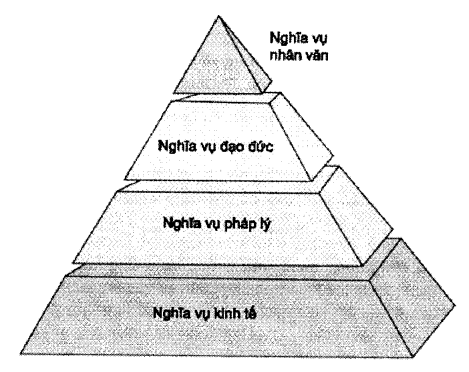
\includegraphics[width=0.8\textwidth]{assert/img2.png}
            \caption{Tháp trách nhiệm xã hội}
            \label{fig:img2}
        \end{figure}

        \begin{itemize}
            \item \textbf{Khía cạnh kinh tế:} 
            
            \qquad Khía cạnh kinh tế trong trách nhiệm xã hội của một doanh nghiệp là phải sản xuất hàng hóa và dịch vụ mà xã hội cần và muốn với một mức giá có thể duy trì doanh nghiệp ấy và làm thỏa mãn nghĩa vụ của doanh nghiệp với các nhà đầu tư; là tìm kiếm nguồn cung ứng lao động, phát hiện những nguồn tài nguyên mới, thúc đẩy tiến bộ công nghệ, phát triển sản phẩm; là phân phối các nguồn sản xuất như hàng hoá và dịch vụ như thế nào trong hệ thống xã hội.

            \qquad Trong khi thực hiện các công việc này, các doanh nghiệp thực sự góp phần vào tăng thêm phúc lợi cho xã hội, đảm bảo sự tồn tại và phát triển của doanh nghiệp. Đối với người lao động, khía cạnh kinh tế của doanh nghiệp là tạo công ăn việc làm với mức thù lao xứng đáng cơ hội việc làm như nhau, cơ hội phát triển nghề và chuyên môn, hưởng thù lao tương xứng, hưởng môi trường lao động an toàn, vệ sinh và đảm bảo quyền riêng tư, cá nhân ở nơi làm việc. Đối với người tiêu dùng, trách nhiệm kinh tế của doanh nghiệp là cung cấp hàng hoá và dịch vụ, trách nhiệm kinh tế của doanh nghiệp còn liên quan đến vấn đề về chất lượng, an toàn sản phẩm, định giá, thông tin về sản phẩm (quảng cáo), phân phối, bán hàng và cạnh tranh. Đối với chủ sở hữu doanh nghiệp, trách nhiệm kinh tế của doanh nghiệp là bảo tồn và phát triển các giá trị và tài sản được uỷ thác. Những giá trị và tài sản này có thể là của xã hội hoặc cá nhân được họ tự nguyện giao phó cho tổ chức, doanh nghiệp - mà đại diện là người quản lý, điều hành - với những điều kiện ràng buộc chính thức. Đối với các bên liên đới khác, nghĩa vụ kinh tế của doanh nghiệp là mang lại lợi ích tối đa và công bằng cho họ. Nghĩa vụ này được thực hiện bằng việc cung cấp trực tiếp những lợi ích cho họ qua hàng hoá, việc làm, giá cả, chất lượng, lợi nhuận đầu tư, v.v...

            \qquad Khía cạnh kinh tế trong trách nhiệm xã hội của một doanh nghiệp là cơ sở cho các hoạt động của doanh nghiệp. Phần lớn các nghĩa vụ kinh tế trong kinh doanh đều được thể chế hoá thành các nghĩa vụ pháp lý.

            \item \textbf{Khía cạnh pháp lý:}
            
            \qquad Khía cạnh pháp lý trong trách nhiệm xã hội của một doanh nghiệp là doanh nghiệp phải thực hiện đầy đủ những quy định về pháp lý chính thức đối với các bên hữu quan. Những điều luật như thế này sẽ điều tiết được cạnh tranh, bảo vệ khách hàng, bảo vệ môi trường, thúc đẩy sự công bằng, an toàn và cung cấp những sáng kiến chống lại những hành vi sai trái. Các nghĩa vụ pháp lý được thể hiện trong luật dân sự và hình sự. Về cơ bản, nghĩa vụ pháp lý bao gồm năm khía cạnh: (1) điều tiết cạnh tranh; (2) bảo vệ người tiêu dùng; (3) bảo vệ môi trường; (4) an toàn và bình đẳng, (5) khuyến khích phát hiện và ngăn chặn hành vi sai trái.

            \qquad Thông qua trách nhiệm pháp lí, xã hội buộc các thành viên phải thực thi các hành vi được chấp nhận. Các tổ chức không thể tồn tại lâu dài nếu họ không thực hiện trách nhiệm pháp lý của mình.

            \item \textbf{Khía cạnh đạo đức:}
            
            \qquad Khía cạnh đạo đức trong trách nhiệm xã hội của một doanh nghiệp là những hành vi và hoạt động mà xã hội mong đợi ở doanh nghiệp nhưng không được quy định trong hệ thống luật pháp, không được thể chế hóa thành luật. Khía cạnh này liên quan tới những gì các công ty quyết định là đúng, công bằng vượt qua cả những yêu cầu pháp lý khắc nghiệt, nó chỉ những hành vi và hoạt động mà các thành viên của tổ chức, cộng đồng và xã hội mong đợi từ phía các doanh nghiệp dù cho chúng không được viết thành luật. Các công ty phải đối xử với các cổ đông và những người có quan tâm trong xã hội bằng một cách thức có đạo đức vì làm ăn theo cách thức phù hợp với các tiêu chuẩn xã hội và những chuẩn tắc đạo đức là vô cùng quan trọng. Vì đạo đức là một phần của trách nhiệm xã hội nên chiến lược kinh doanh cần phải phản ánh tầm hiểu biết, tầm nhìn về các giá trị của các thành viên trong tổ chức và các cổ đông và hiểu biết về bản chất đạo đức của những sự lựa chọn mang tính chiến lược. Khía cạnh đạo đức của một doanh nghiệp thường được thể hiện thông qua những nguyên tắc, giá trị đạo đức được tôn trọng trình bày trong bản sứ mệnh và chiến lược của công ty. Thông qua các công bố này, nguyên tắc và giá trị đạo đức trở thành kim chỉ nam cho sự phối hợp hành động của mỗi thành viên trong công ty với các bên hữu quan.

            \item \textbf{Khía cạnh nhân văn (Lòng bác ái):}
            
            \qquad Khía cạnh nhân văn trong trách nhiệm xã hội của một doanh nghiệp là những hành vi và hoạt động thể hiện những mong muốn đóng góp và hiến dâng cho cộng đồng và xã hội. Ví dụ như, thành lập các tổ chức từ thiện và ủng hộ các dự án cộng đồng là hình thức thể hiện lòng bác ái và tinh thần tự nguyện của công ty đó.

            \qquad Những đóng góp có thể trên bốn phương diện: Nâng cao chất lượng cuộc sống, san sẻ bớt gánh nặng cho chính phủ, nâng cao năng lực lãnh đạo cho nhân viên và phát triển nhân cách đạo đức của người lao động.

            \qquad Khía cạnh này liên quan tới những đóng góp về tài chính và nguồn nhân lực cho cộng đồng và xã hội lớn hơn để nâng cao chất lượng cuộc sống. Khía cạnh nhân ái của trách nhiệm pháp lý liên quan tới cơ cấu và động lực của xã hội và các vấn đề về chất lượng cuộc sống mà xã hội quan tâm. Người ta mong đợi các doanh nghiệp đóng góp cho cộng đồng và phúc lợi xã hội. Các công ty đã đóng góp những khoản tiền đáng kể cho giáo dục, nghệ thuật, môi trường và cho những người khuyết tật. Các công ty không chỉ trợ giúp các tổ chức từ thiện địa phương và trên cả nước mà họ còn tham gia gánh vác trách nhiệm giúp đào tạo những người thất nghiệp. Lòng nhân ái mang tính chiến lược kết nối khả năng của doanh nghiệp với nhu cầu của cộng đồng và của xã hội.

            \qquad Đây là thứ trách nhiệm được điều chỉnh bởi lương tâm. Chẳng ai có thể bắt buộc các doanh nghiệp phải bỏ tiền ra để xây nhà tình nghĩa hoặc lớp học tình thương, ngoài những thôi thúc của lương tâm. Tuy nhiên, thương người như thể thương thân là đạo lý sống ở đời. Nếu đạo lý đó ràng buộc mọi thành viên trong xã hội thì nó không thể không ràng buộc các doanh nhân. Ngoài ra, một xã hội nhân bản và bác ái là rất quan trọng cho hoạt động kinh doanh. Bởi vì trong xã hội như vậy, sự giàu có sẽ được chấp nhận. Thiếu điều này, động lực của hoạt động kinh doanh sẽ bị tước bỏ.

        \end{itemize}

        \vspace{0.2cm}
        Dưới đây, chúng ta sẽ kiểm định 4 thành tố của trách nhiệm xã hội: Thông qua trách nhiệm pháp lý - cơ sở khởi đầu của mọi hoạt động kinh doanh, xã hội buộc các thành viên phải thực thi các hành vi được chấp nhận. Các tổ chức không thể tồn tại lâu dài nếu họ không thực hiện trách nhiệm pháp lí của mình. Bước tiếp theo mà các tổ chức cần lưu tâm là trách nhiệm đạo đức. Các công ty phải quyết định những gì họ cho là đúng, chính xác và công bằng theo những yêu cầu nghiêm khắc của xã hội. Nhiều người xem pháp luật chính là những đạo đức được hệ thống hoá. Sau sự quyết định tại thời điểm này có thể sẽ trở thành luật lệ trong tương lai nhằm cải thiện tư cách công dân của tổ chức. Trong việc thực thi trách nhiệm pháp lý và trách nhiệm xã hội của mình, các tổ chức cũng phải chú trọng tới những mối quan tâm về kinh tế của các cổ đông. Thông qua hành vi pháp lý và đạo đức thì tư cách công dân tốt sẽ mang lại lợi ích lâu dài. Bước cuối cùng của trách nhiệm xã hội là trách nhiệm về lòng bác ái. Bằng việc thực thi trách nhiệm về lòng bác ái, các công ty đóng góp các nguồn lực về tài chính và nhân lực cho cộng đồng để cải thiện chất lượng cuộc sống. Khía cạnh lòng bác ái và kinh tế của trách nhiệm xã hội có mối liên hệ mật thiết với nhau, bởi vì tổ chức càng làm được nhiều lợi nhuận bao nhiêu thì cơ hội họ đầu tư vào các hoạt động nhân đức càng lớn bấy nhiêu. Mỗi khía cạnh của trách nhiệm xã hội định nghĩa một lĩnh vực mà các công ty phải đưa ra quyết định biểu thị dưới dạng những hành vi cụ thể sẽ được xã hội đánh giá.

\subsection{Cách thức thực hiện}
    \begin{enumerate}[a.]
        % Voi lenh \setcounter{enumi}{x}
        % with x = 1, 2, 3, ...
        % enum_ voi _ la chu so La Ma chi cap cua cay item enumerate
        % danh so bat dau tu x + 1
        % anh xa 1 - a - i; 2 - b - ii; 3 - c - iii
        \item \textbf{Xây dựng bộ quy tắc đạo đức}
        \begin{itemize}
            \item Thiết lập và công bố bộ quy tắc đạo đức kinh doanh rõ ràng.
            \item Định nghĩa các nguyên tắc về trung thực, minh bạch, công bằng, trách nhiệm đối với khách hàng, nhân viên và cộng đồng.
            \item Yêu cầu tất cả nhân viên và đối tác tuân thủ bộ quy tắc này.
        \end{itemize}
        \item \textbf{Đào tạo và tuyên truyền về đạo đức kinh doanh}
        \begin{itemize}
            \item Tổ chức các buổi đào tạo định kỳ cho nhân viên về đạo đức nghề nghiệp, chống tham nhũng, bảo mật thông tin
            \item Tạo môi trường làm việc khuyến khích hành vi đạo đức và tinh thần trách nhiệm xã hội.
            \item Xây dựng văn hóa doanh nghiệp dựa trên các giá trị cốt lõi về đạo đức.
        \end{itemize}
        \item \textbf{Minh bạch và trung thực trong kinh doanh}
        \begin{itemize}
            \item Cung cấp thông tin đầy đủ, rõ ràng về sản phẩm, dịch vụ và tài chính.
            \item Đảm bảo các báo cáo tài chính được kiểm toán chặt chẽ và chính xác.
            \item Không tham gia vào các hoạt động gian lận, lừa đảo, cạnh tranh không lành mạnh.
        \end{itemize}  
        \item \textbf{Áp dụng công nghệ xanh, sản xuất bền vững}
        \begin{itemize}
            \item Sử dụng công nghệ thân thiện với môi trường, giảm thiểu khí thải và rác thải công nghiệp.
            \item Tận dụng năng lượng tái tạo và nguyên liệu sinh thái trong sản xuất.
            \item Hạn chế sử dụng nhựa, tăng cường tái chế và quản lý chất thải hiệu quả.
        \end{itemize}
        \item \textbf{Đảm bảo quyền lợi và phúc lợi cho nhân viên}
        \begin{itemize}
            \item Xây dựng môi trường làm việc công bằng, an toàn và không phân biệt đối xử.
            \item Cung cấp chế độ lương thưởng, bảo hiểm và phúc lợi hợp lý cho nhân viên.
            \item Khuyến khích sự cân bằng giữa công việc và cuộc sống cá nhân.
        \end{itemize}
        \item \textbf{Tham gia các hoạt động cộng đồng và từ thiện}
        \begin{itemize}
            \item Đóng góp tài chính hoặc hỗ trợ nhân lực cho các tổ chức từ thiện, giáo dục và y tế.
            \item Khuyến khích nhân viên tham gia tình nguyện, hoạt động vì cộng đồng.
            \item Tổ chức hoặc tài trợ các sự kiện mang lại lợi ích cho xã hội.
        \end{itemize}
        \item \textbf{Tuân thủ pháp luật và các quy định hiện hành}
        \begin{itemize}
            \item Luôn tuân theo các quy định pháp luật về lao động, thuế, môi trường, an toàn thực phẩm,...
            \item Hợp tác chặt chẽ với chính phủ và các tổ chức kiểm soát để đảm bảo hoạt động kinh doanh minh bạch và hợp pháp.
        \end{itemize}
        \item \textbf{Tích hợp trách nhiệm xã hội vào chiến lược kinh doanh}
        \begin{itemize}
            \item Không chỉ coi trách nhiệm xã hội là một hoạt động bên lề, mà cần tích hợp vào chiến lược kinh doanh dài hạn.
            \item Xây dựng các sản phẩm, dịch vụ mang lại giá trị cho xã hội và môi trường.
            \item Tạo dựng hình ảnh doanh nghiệp có trách nhiệm và đạo đức để thu hút khách hàng và nhà đầu tư.
        \end{itemize}
    \end{enumerate}

    \vspace{0.2cm}
    Việc thực hiện tốt các phương pháp trên sẽ giúp doanh nghiệp không chỉ duy trì đạo đức kinh doanh mà còn tạo dựng được niềm tin và sự ủng hộ từ khách hàng, đối tác và cộng đồng.

\subsection{Chỉ tiêu đánh giá}
    \begin{figure}[H]
        \centering
        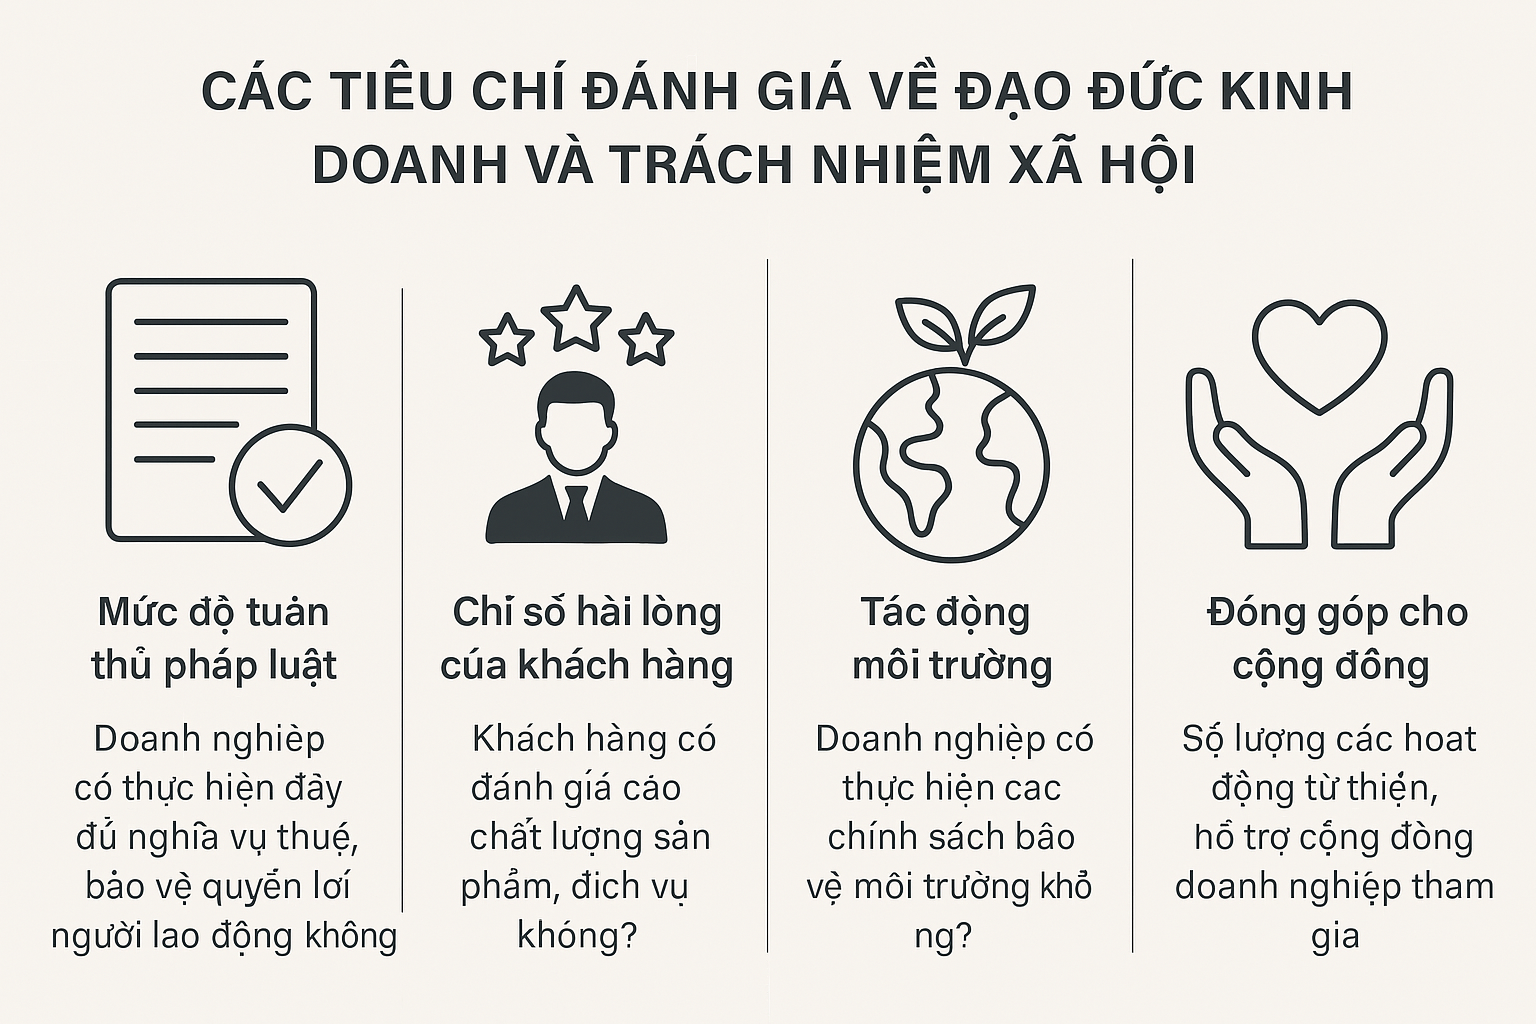
\includegraphics[width=0.8\textwidth]{assert/img3.png}
        \caption{Các tiêu chí đánh giá đạo đức kinh doanh và trách nhiệm xã hội}
        \label{fig:img3}
    \end{figure}

    \begin{enumerate}[a.]
        \item \textbf{Mức độ tuân thủ pháp luật}
        \begin{itemize}
            \item Doanh nghiệp có thực hiện đầy đủ nghĩa vụ thuế không?
            \item Có tuân thủ các quy định về bảo vệ quyền lợi người lao động (hợp đồng lao động, bảo hiểm, giờ làm việc, an toàn lao động,...) không?
            \item Có đảm bảo minh bạch tài chính, không gian lận hay trốn thuế không?
            \item Có tuân thủ các quy định về môi trường, an toàn thực phẩm, sở hữu trí tuệ không?
        \end{itemize}
        \item \textbf{Chỉ số hài lòng của khách hàng}
        \begin{itemize}
            \item Khách hàng có đánh giá cao chất lượng sản phẩm, dịch vụ không?
            \item Doanh nghiệp có thường xuyên cải tiến sản phẩm/dịch vụ để đáp ứng nhu cầu khách hàng không?
            \item Tỷ lệ khiếu nại, phản hồi tiêu cực từ khách hàng có thấp không?
            \item Doanh nghiệp có chính sách chăm sóc khách hàng và giải quyết khiếu nại hợp lý không?
        \end{itemize}
        \item \textbf{Tác động đến môi trường}
        \begin{itemize}
            \item Doanh nghiệp có thực hiện các chính sách bảo vệ môi trường không?
            \item Có áp dụng công nghệ xanh, sản xuất bền vững, tiết kiệm tài nguyên không?
            \item Có kế hoạch quản lý và xử lý chất thải hiệu quả không?
            \item Có sử dụng năng lượng tái tạo, giảm phát thải khí nhà kính không?
        \end{itemize}  
        \item \textbf{Mức độ đảm bảo phúc lợi cho nhân viên}
        \begin{itemize}
            \item Mức lương, chế độ đãi ngộ có công bằng và hợp lý không?
            \item Doanh nghiệp có quan tâm đến sức khỏe, an toàn lao động của nhân viên không?
            \item Môi trường làm việc có chuyên nghiệp, công bằng, không phân biệt đối xử không?
            \item Nhân viên có được đào tạo, phát triển kỹ năng và cơ hội thăng tiến không?
        \end{itemize}
        \item \textbf{Đóng góp cho cộng đồng}
        \begin{itemize}
            \item Doanh nghiệp có tham gia các hoạt động từ thiện, hỗ trợ cộng đồng không?
            \item Có đóng góp cho giáo dục, y tế, phát triển xã hội không?
            \item Có chính sách hỗ trợ các nhóm yếu thế, tạo cơ hội việc làm cho người có hoàn cảnh khó khăn không?
            \item Có tài trợ hoặc tổ chức các chương trình vì lợi ích chung không?
        \end{itemize}
        \item \textbf{Minh bạch và đạo đức trong kinh doanh}
        \begin{itemize}
            \item Doanh nghiệp có công khai thông tin tài chính, hoạt động kinh doanh minh bạch không?
            \item Có tránh các hành vi gian lận, hối lộ, thao túng thị trường không?
            \item Có chính sách chống tham nhũng, đảm bảo công bằng trong hợp tác kinh doanh không?
            \item Có chính sách bảo vệ quyền lợi của cổ đông và nhà đầu tư không?
        \end{itemize}
        \item \textbf{Mức độ gắn kết với các bên liên quan}
        \begin{itemize}
            \item Doanh nghiệp có duy trì quan hệ tốt với đối tác, nhà cung cấp không?
            \item Có hợp tác bền vững, công bằng với các bên liên quan không?
            \item Có lắng nghe phản hồi và giải quyết thỏa đáng các vấn đề phát sinh không?
        \end{itemize}
        \item \textbf{Chứng nhận và xếp hạng về đạo đức kinh doanh và trách nhiệm xã hội}
        \begin{itemize}
            \item Doanh nghiệp có được các tổ chức uy tín cấp chứng nhận về trách nhiệm xã hội (CSR), môi trường (ISO 14001), lao động (SA 8000),... không?
            \item Có được xếp hạng cao trong các bảng xếp hạng doanh nghiệp bền vững không?
        \end{itemize}
    \end{enumerate}

    \vspace{0.2cm}
    Một doanh nghiệp đáp ứng tốt các tiêu chí trên có thể được đánh giá là có nền tảng đạo đức kinh doanh vững chắc và thực hiện tốt trách nhiệm xã hội.

% ========================= Phần 2 ==========================
\newpage
\section{Phân tích về doanh nghiệp Coca-Cola}
\subsection{Giới thiệu về doanh nghiệp Coca-Cola}
    \subsubsection{Coca-Cola là gì?}
    \vspace{0.2cm}
    \textbf{Coca-Cola} (thường được nói tắt là \textbf{Coca}) là một thương hiệu nước ngọt có ga chứa nước cacbon điôxít bão hòa được sản xuất bởi Công ty Coca-Cola. Coca-Cola ban đầu được điều chế bởi dược sĩ John Pemberton vào cuối thế kỷ XIX với mục đích trở thành một loại biệt dược. Tuy nhiên, doanh nhân người Mỹ Asa Griggs Candler sau đó đã mua lại công thức loại thuốc uống này, và bằng những chiến thuật tiếp thị thông minh, ông đã đưa Coca-Cola trở thành một trong những sản phẩm dẫn đầu thị trường nước ngọt có ga trong thế kỷ XX. Tên của Coca-Cola bắt nguồn từ hai thành phần nguyên bản của thức uống này: hạt côla (chứa nhiều caffein) và lá cây côca. Hiện nay, công thức Coca-Cola vẫn còn là một bí mật thương mại, dù cho nhiều công thức thử nghiệm khác nhau đã được công bố rộng rãi.

    \vspace{0.2cm}
    Công ty Coca-Cola sẽ chịu trách nhiệm sản xuất phần chất lỏng cô đặc. Phần nước này sau đó sẽ được bán cho các nhà máy đóng chai Coca-Cola có giấy phép kinh doanh trên khắp thế giới. Các nhà máy này đã có hợp đồng độc quyền theo từng khu vực với công ty, và sẽ tiếp tục hoàn thành sản phẩm bằng cách đóng lon hoặc chai đựng chất cô đặc kèm với nước đã qua xử lý và các chất tạo ngọt. Một lon Coca-Cola 1.2 oz cơ bản ở Mỹ (tức lon 350 ml) có thể chứa tới 38 gram (tức 1,3 oz) đường (thường ở dưới dạng đường HFCS). Các loại Coca-Cola đóng chai sau đó sẽ được bày bán, phân phối và vận chuyển tới các cửa hàng bán lẻ, nhà hàng và máy bán hàng tự động trên toàn thế giới. Công ty Coca-Cola ngoài ra cũng bán phần chất cô đặc cho các thùng chứa nước ngọt tại các nhà phân phối dịch vụ thực phẩm và các nhà hàng lớn.

    \subsubsection{Lịch sử hình thành của doanh nghiệp Coca-Cola}
        \paragraph{Lịch sử của công ty Coca-Cola trên toàn cầu}
        \begin{itemize}
            \item Cha đẻ của Coca-Cola là dược sỹ người Mỹ John S. Pemberton. Sản phẩm lần đầu tiên được giới thiệu đến công chúng ở Atlanta vào 5/8/1886. Ban đầu Coca-Cola được người Mỹ biết đến như một loại thuốc uống. 
            \item Vào năm 1891, Asa G.Candler (thương gia người Atlanta) nhận ra tiềm năng to lớn của Coca-Cola nên ông quyết định mua lại công thức cũng như toàn bộ quyền sở hữu  Coca-Cola với giá 2,300 USD. (Biến chuyển suy nghĩ của người tiêu dùng từ 1 thứ thuốc uống thành 1 đồ uống ngon lành và tươi mát)
            \item 1892 Công ty Coca-Cola được thành lập. Một năm sau, nó chính thức được đăng kí quyền sở hữu công nghiệp.
            \item Vào năm 1919,  Coca-Cola được bán cho Ernest Woodruff ( chủ 1 ngân hàng ở Atlanta)
            \item Sau hơn 1 thế kỷ được thành lập và phát triển Coca-Cola đã có mặt ở hơn 200 quốc gia trên thế giới trong đó có Việt Nam.
            \item Đại gia đình Coca-Cola toàn cầu vẫn luôn giữ vững vị thế đứng đầu toàn cầu trong ngành công nghiệp giải nước giải khát. Coca-Cola vẫn luôn phản chiếu những bước chuyển của thời gian, luôn bắt nhịp với những đổi thay chưa từng thấy của toàn cầu.
            \item Ngày nay, Coca-Cola đã rất thành công trong chiến lược mở rộng thị trường với nhiều loại nước uống khác nhau: ban đầu là nước có gas, sau đó là nước trái cây, nước tăng lực, nước suối và một số loại khác.
        \end{itemize}
        \paragraph{Lịch sử của Coca-Cola tại Việt Nam}
        \begin{itemize}
            \item 1960, Coca-Cola lần đầu tiên được giới thiệu tại Việt Nam.
            \item 1994 trở lại VN và bắt đầu kinh doanh
            \item 8/1995: Liên doanh với công ty Vinafimex, đặt trụ sở tại miền bắc
            \item 9/1995: Liên doanh với công ty Chương Dương Việt Nam, đặt trụ sở tại Miền Nam
            \item 1/1998: Liên doanh với cty nước giải khát Đà Nẵng, đặt trụ sở tại Miền Trung
            \item 6/2001: Hợp nhật thành Coca-Cola Việt Nam
            \item 1/3/2004: Coca-Cola Việt Nam được chuyển giao cho Sabco - 1 trong những tập đoàn đóng chai danh tiếng của Coca-Cola trên thế giới.
        \end{itemize}

    \subsubsection{Logo của Coca-Cola}
    \begin{figure}[H]
        \centering
        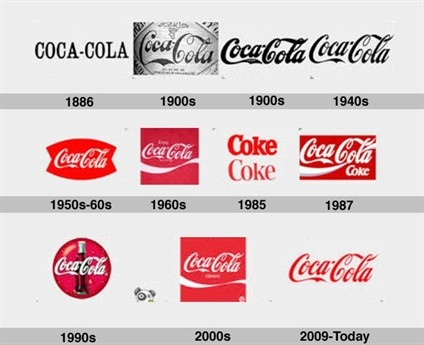
\includegraphics[width=0.8\textwidth]{assert/img4.jpg}
        \caption{Tổng hợp các logo của Coca-Cola, từ 1886 đến nay}
        \label{fig:img4}
    \end{figure}

    \vspace{0.2cm}
    \textbf{Logo của Coca-Cola} được thiết kế bởi một người nghiệp dư, Frank Robinson, ông là nhân viên kế toán mới vào nghề của công ty. Logo của Coca-Cola gần như là một trong những logo đình đám nhất cho làng giải khát.

    \vspace{0.2cm}
    Từ năm 1886 đến năm 2007, logo Coca-Cola đã có 12 phiên bản khác nhau. Ban đầu, logo Coke lấy màu đen làm màu sắc chủ đạo. Sắc đỏ trắng phải đến tận năm 1950 mới được xuất hiện và trở thành nền tảng cho các phiên bản logo về sau.

    \vspace{0.2cm}
    Màu sắc đỏ và trắng trong logo của Coca-Cola là đủ đơn giản, vui tươi và đặc biệt để thu hút khán giả trẻ. Trong khi màu đỏ tượng trưng cho niềm đam mê, sự quyết tâm, sự trẻ trung và sức sống, màu trắng tượng trưng cho sự quyến rũ và sang trọng của thương hiệu Coca-Cola.

    \vspace{0.2cm}
    Tuy thiết kế của logo Coca-Cola hiện nay theo phong cách đơn giản nhưng chính những nét lượn sóng cùng với sắc đỏ trắng đã để lại ấn tượng mạnh trong lòng công chúng. Đó chính là những dấu ấn làm nên thương hiệu của Coca-Cola.

\subsection{Những hiệu quả và thành tựu của Coca-Cola}
    \subsubsection{Những hiệu quả mà Coca-Cola đã đạt được}
    \vspace{0.2cm}
    Coca-Cola đã có những thành công nhất định trong việc xây dựng thương hiệu và tạo dựng lòng tin với người tiêu dùng. Một số hiệu quả mà Coca-Cola đã đạt được bao gồm:
    \begin{itemize}
        \item Luôn đem lại cảm giác an toàn và tiện lợi cho người tiêu dùng. Điều này vô cùng quan trọng đối với một sản phẩm được bày bán rộng rãi trên thị trường. Chính chất lượng sản phẩm của Coca-Cola đã chinh phục được khách hàng, từ đó tạo lòng tin và thúc đẩy hiệu quả kinh doanh.
        \item Truyền tải tinh thần lạc quan, yêu đời cho người tiêu dùng bằng cách thông qua những quảng cáo và slogan. Coca đã truyền cảm hứng cho rất nhiều khách hàng ở mọi độ tuổi.
        \item Tạo nên những thay đổi tích cực là làm cho giá trị cuộc sống ngày càng ý nghĩa hơn
    \end{itemize}

    $\Rightarrow$ Một trong những cách mà Coca-Cola luôn giữ vững được mối quan hệ tốt đẹp với người tiêu dùng chính là luôn hòa nhập vào hoạt động của họ. Các tổ chức các hoạt động quảng bá thương hiệu của Coca-Cola đã góp phần đưa thương hiệu này đến tay người tiêu dùng một cách nhanh chóng và hiệu quả nhất. Qua đó càng chứng tỏ Coca-Cola đang là một loại nước uống có chất lượng tốt, luôn có chỗ đứng vững chắc và chiếm lĩnh được thị phần trên thị trường vượt trội hơn so với các nhãn hiệu nước ngọt khác.

    \subsubsection{Những thành tựu mà Coca-Cola đã đạt được}
    \vspace{0.2cm}
    Từ khi được thành lập và đặt trụ sở chính tại Atlanta, bang Georgia, tập đoàn Coca-Cola hiện đang hoạt động trên 200 nước khắp thế giới. Thương hiệu Coca-Cola luôn là thương hiệu nước ngọt bán chạy hàng đầu và tất cả mọi người trên thế giới đều yêu thích Coca-Cola hoặc một trong những loại nước uống hấp dẫn khác của tập đoàn. Ngày nay, tập đoàn Coca-Cola đã thành công trong công cuộc mở rộng thị trường với nhiều loại nước uống khác nhau ban đầu là nước có gas, và sau đó là nước trái cây, nước tăng lực cho thể thao, nước suối, trà và một số loại khác.
    
    \vspace{0.2cm}
    Coca-Cola chiếm 3.1\% tổng lượng sản phẩm thức uống trên toàn thế giới. Trong 33 nhãn hiệu nước giải khát không cồn nổi tiếng trên thế giới, Coca-Cola sở hữu tới 15 nhãn hiệu. Mỗi ngày Coca-Cola bán được hơn 1 tỷ loại nước uống, mỗi giây lại có hơn 10.000 người dùng sản phẩm của Coca-Cola. Trung bình một người Mỹ uống sản phẩm của công ty Coca-Cola 4 ngày 1 lần. Coca-Cola hiện đã có mặt tại tất cả các châu lục trên thế giới và được biết đến rộng rãi bởi phần lớn dân số thế giới.

    \vspace{0.2cm}
    Năm 2007, Coca-Cola đã trả cho các nhà cung cấp nguyên vật liệu là 11 tỷ USD và tiền lương cho 73.000 công nhân là gần 4 tỷ USD. Sản xuất tiêu thụ hết 36 triệu lít nước, 6 tỷ J (Joule/Jun) năng lượng. Có khoảng 1.2 triệu các nhà phân phối sản phẩm của Coca-Cola, 2.4 triệu máy bán lẻ tự động, nộp 1.4 tỷ USD tiền thuế và đầu tư cho cộng đồng 31.5 triệu USD.

    \vspace{0.2cm}
    $\Rightarrow$ Coca-Cola đã trở thành một trong những thương hiệu nổi tiếng nhất trên thế giới, với giá trị thương hiệu ước tính lên tới 83 tỷ USD. Coca-Cola không chỉ là một loại nước giải khát mà còn là biểu tượng của sự lạc quan và niềm vui sống.

\subsection{Một số đạo đức kinh doanh của Coca-Cola}
    \subsubsection{Đưa ra những chiến lược marketing hiệu quả, phù hợp với nhu cầu của người tiêu dùng.}
    \vspace{0.2cm}
    Chiến lược marketing của Coca-Cola được biểu hiện qua 6 phương diện
    \begin{itemize}
        \item \textbf{Chất lượng sản phẩm:}
        
        \qquad Tất cả sản phẩm của Coca-Cola, từ nước giải khát có ga, nước đóng chai đến nước giải khát có bổ sung vi chất dinh dưỡng như Nutriboost, Teppy, Aquarius, Dasani có bổ sung khoáng chất, Coca-Cola đều có giấy tiếp nhận công bố đạt tiêu chuẩn chất lượng sản phẩm của Bộ Y tế. Không chỉ vậy, kết quả kiểm nghiệm của các sản phẩm đều cho thấy chỉ tiêu chất lượng phù hợp với tiêu chuẩn đã được công bố. Do đó, người tiêu dùng có thể an tâm sử dụng. Mỗi sản phẩm đến tay người tiêu dùng đều đảm bảo được 2 tiêu chí: chất lượng và an toàn.

        \qquad Bằng việc tuân thủ nghiêm ngặt các cam kết với người tiêu dùng, quy trình quản lý chất lượng sản phẩm chuẩn quốc tế cùng những giá trị cộng đồng tạo dựng được, Coca-Cola thật sự nỗ lực và quyết tâm mang đến nhiều điều tốt đẹp hơn cho người tiêu dùng. Coca-Cola chủ yếu cải tiến để đảm bảo vệ sinh an toàn thực phẩm.
        \item \textbf{Nhãn hiệu:}
        
        \qquad Coca-Cola đã luôn là một phần không thể thiếu được trong các sự kiện lớn ở Mỹ và khắp trên toàn thế giới. Tính đến nay, CocaCola đã cho ra mắt hơn 300 nhãn hiệu nước giải khát khác nhau ở các nước trên thế giới (Trừ Cuba và CHDCND Triều Tiên).

        \qquad Coca-Cola áp dụng đặt tên nhãn hiệu cho từng sản phẩm riêng biệt. Ví dụ: Fanta, Samurai (Hiện đã ngừng sản xuất), Sprite, 7UP...

        \quad $\Rightarrow$ Điều này khiến cho người tiêu dùng có thể dễ đọc, dễ nhận dạng, dễ nhớ hơn. Nhãn hiệu của Coca-Cola luôn gây được ấn tượng mạnh và quan trọng là Coca đang trên đà phát triển để đa dạng hóa danh mục sản phẩm. Nhãn hiệu Coca tạo ra làm liên tưởng đến bọt gas trắng và màu nước đặc trưng, chính vì vậy đã tạo nên khác biệt với sản phẩm khác trên thị trường.
        \item \textbf{Bao bì:}
        
        \qquad Từ khi thành lập màu sắc đặc trưng cho Coca Cola đó chính là màu đỏ, dựa vào màu đỏ sẽ giúp họ nhận dạng cửa hàng cũng như dễ dàng tìm kiếm sản phẩm hơn giữa rất nhiều sản phẩm cùng loại. Mặc dù, sau này có nhiều sản phẩm khác nhau và có màu sắc riêng biệt nhưng khách hàng vẫn có thể dựa vào những màu sắc đặc trưng cho từng loại sản phẩm. Tiêu biểu như màu đỏ của loại Coca Cola truyền thống, màu trắng của Diet Coke, màu xanh Sprite, màu cam Fanta. Với những màu sắc quen thuộc sẽ giúp cho khách hàng dễ dàng nhận ra sản phẩm của thương hiệu này mà không cần phải đọc kỹ các thông tin trên bao bì sản phẩm.

        \qquad Bao bì Coca-Cola vào những dịp lễ tết còn tôn vinh những khoảnh khắc yêu thương, gắn kết. Đối với tình yêu gia đình vốn được đề cao và trân trọng trong những dịp Tết đến, Coca-Cola cùng họa sĩ Đạt Phan đã khắc họa khoảnh khắc sum vầy của các thành viên thông qua hình ảnh đoàn tụ của gia đình chim én. Với đôi cánh dang rộng và ánh nhìn trìu mến dành cho đàn con, gia đình én đã góp phần tạo nên không khí sum họp, đầm ấm mùa Tết. Bên cạnh đó, Coca-Cola cùng với sự hợp tác của Mr.Smith đã bổ sung vào bộ sưu tập “Tết của yêu thương” một bức tranh tình yêu đẹp đẽ của đôi én Xuân, nhắn nhủ một mùa yêu bùng cảm xúc. Và thiết kế Coca-Cola Tết tình yêu cộng đồng là sự hội tụ của những cánh én từ 3 miền đất nước, mang lộc Xuân trải khắp mọi nơi, đem lại một mùa Tết vẹn tròn yêu thương.

        \qquad \textbf{Màu sắc chủ yếu trên bao bì Coca-Cola là màu đỏ. Đó cũng là màu chủ đạo trong nhiều logo trong lịch sử của Coca-Cola}

        \begin{figure}[H]
            \centering
            \begin{minipage}{0.4\textwidth}
                \centering
                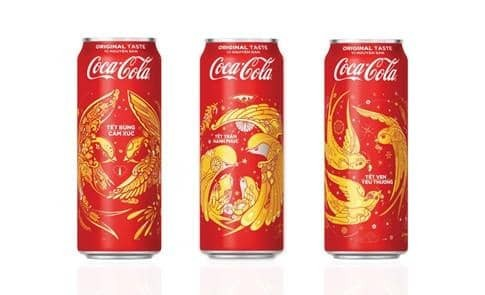
\includegraphics[width=\textwidth]{assert/img51.jpg}
            \end{minipage}
            \begin{minipage}{0.4\textwidth}
                \centering
                
\includegraphics[width=\textwidth]{assert/img52.jpg}
            \end{minipage}
            \label{fig:img5}
            \caption{Bao bì của Coca-Cola vào dịp Tết 2018}
        \end{figure}
        \item \textbf{Giá cả:}
        
        \qquad Về phần giá cả, Coca-Cola luôn bám sát biến động của thị trường nhằm đảm bảo tính cạnh tranh, đồng thời vẫn duy trì được chất lượng sản phẩm của mình và lợi nhuận hợp lý cho các bên phân phối.
        
        \qquad Coca-Cola định giá theo phương pháp cạnh tranh :giá của Coca-Cola ngang bằng hoặc hơi cao hơn với giá của Pepsi. Giá cả các sản phẩm của Coca-Cola cũng như giá của thị trường nước giải khát tăng đều theo sự tăng lên của thu nhập người dân và sự lạm phát.
        
        \qquad Sau đây là bảng giá Coca-Cola tại một sỉ lớn, năm 2023:
        \begin{figure}[H]
            \centering
            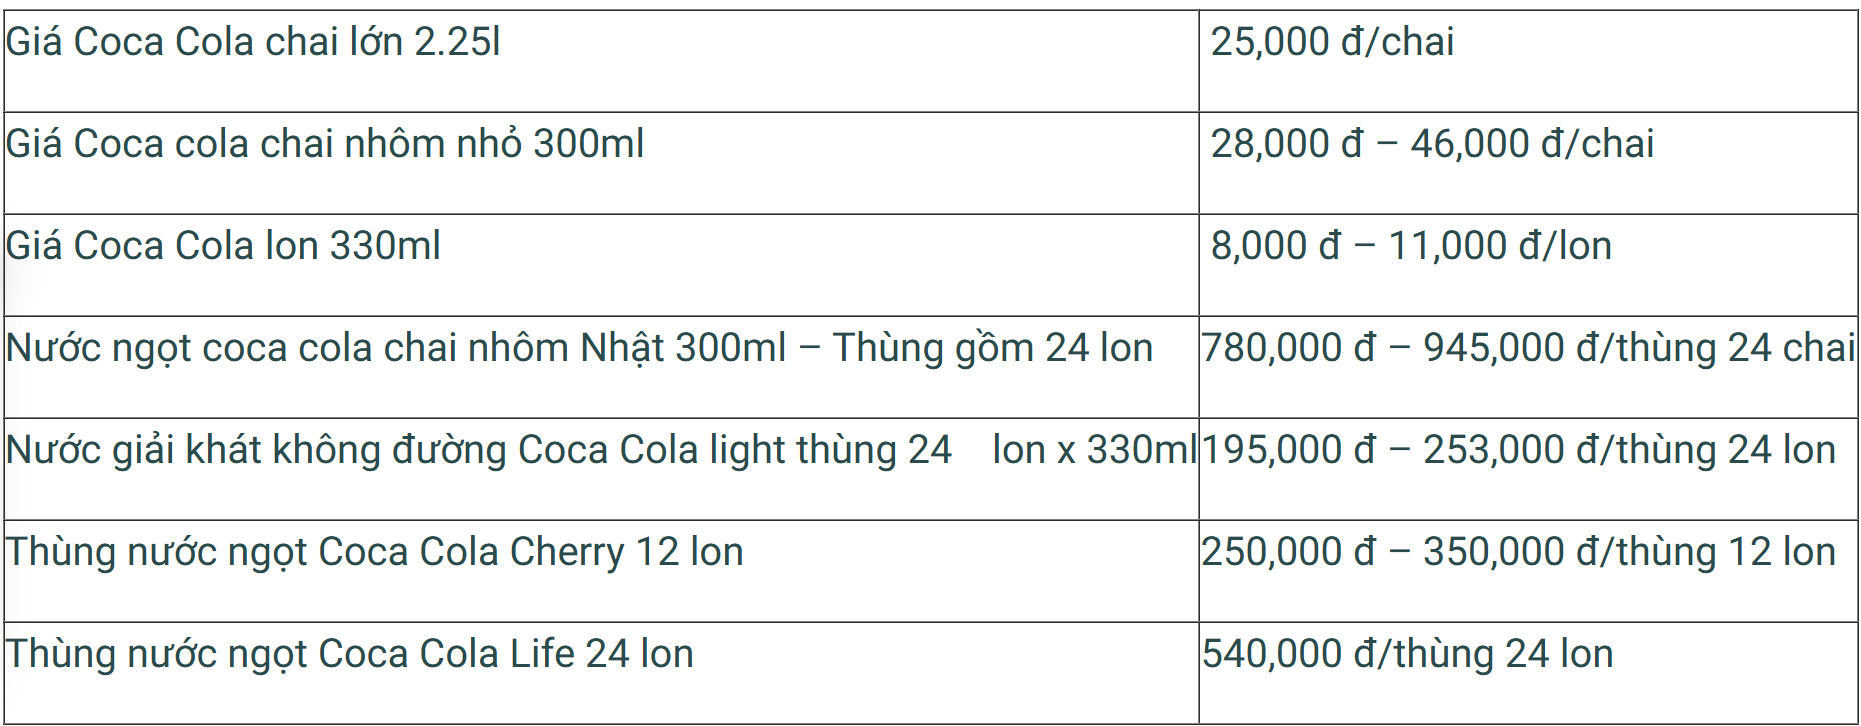
\includegraphics[width=0.9\textwidth]{assert/img6.png}
            \caption{Bảng giá Coca-Cola tại một sỉ lớn, năm 2023, đã bao gồm VAT}
            \caption*{(Nguồn: \href{https://www.gufoods.com/bang-gia-nuoc-ngot-moi-nhat-thi-truong-tet-2023}{https://www.gufoods.com/bang-gia-nuoc-ngot-moi-nhat-thi-truong-tet-2023})}
            \label{fig:img6}
        \end{figure}

        \item \textbf{Phân phối:}
        
        Coca-Cola có một hệ thống phân phối rất mạnh mẽ và rộng khắp. Hệ thống phân phối của Coca-Cola được chia thành các cấp như sau:
        \begin{itemize}
            \item \textbf{CÔNG TY SẢN XUẤT:} Công ty Coca Cola nói chung được chia thành hai bộ phận, hai hoạt động riêng biệt đó là:
            \begin{itemize}
                \item TCC (The Coca Cola Company): chịu trách nhiệm sản xuất và cung cấp nước cốt Coca-Cola cho các nhà máy mà chịu trách nhiệm khuếch trương và quản lý thương hiệu.
                \item TCB (The Coca Cola Bottler): chịu trách nhiệm sản xuất, dự trữ kho bãi, phân phối và cung cấp dịch vụ cho sản phẩm Coca Cola.
            \end{itemize}
            \item \textbf{DOANH NGHIỆP TRUNG TÂM:} Trụ sở chính và cũng là trung tâm phân phối lớn nhất của Coca-Cola nằm ở AtLanta, Georgia, hoa kỳ. Và công ty phân phối hấu hết các quốc gia trên khắp thế giới.
            \item \textbf{NHÀ PHÂN PHỐI:} các nhà phân phối của Coca-Cola được chia thành 2 loại:
            \begin{itemize}
                \item Các nhà bán buôn sẽ thực hiện các chức năng phân phối vật chất, vận chuyển, bảo quản, dự trữ tồn kho với số lượng lớn, sắp xếp và phân loại hàng hóa, đặt và nhận các đơn đặt hàng, thông tin và bán hàng.
                \item Nhà buôn bán thường phân phối cho các nhà bán lẻ, từ các cửa hàng nhỏ đến các bách hóa lớn. Họ cũng có thể phân phối cho các nhà hàng, quán bar, khách sạn và các cơ sở dịch vụ ăn uống khác.
            \end{itemize}
            \item \textbf{BÁN LẺ:} Các cam kết, thỏa thuận từ Coca Cola với các nhà bán lẻ có thể là trực tiếp hoặc là thông qua các nhà bán buôn nhưng đều phải thực hiện chặt chẽ và tuân theo các quy định có sẵn.
            \item \textbf{NGƯỜI TIÊU DÙNG:} Là những cá nhận, tổ chức tiêu thụ sản phẩm, trực tiếp sử dụng sản phẩm của Coca Cola. Họ tạo nên thị trường mục tiêu của công ty và chính họ là những người ảnh hưởng trực tiếp tới doanh số của công ty.
        \end{itemize}
        \item \textbf{Xúc tiến:}
        \begin{enumerate}[a.]
            \item \textbf{Về phần quảng cáo:}
            \begin{itemize}
                \item Mục tiêu quảng cáo của Coca-Cola:
                \begin{itemize}
                    \item Thông báo cho thị trường về các sản phẩm mới.
                    \item Duy trì mức độ tiếp cận ở mức độ cao, mong muốn được nhiều khách hàng biết đến sản phẩm.
                \end{itemize}
                \item Quyết định ngân sách quảng cáo của Coca-Cola: Đối với ngân sách quảng cáo, Coca-Cola luôn đặt ra những chiến lược nhất định, quan trọng là phải phù hợp với nội dung quảng cáo, hình thức quảng cáo.
                \item Quyết định thông điệp quảng cáo: Coca-Cola luôn đem lại 2 thông điệp chính trong từng sản phẩm.
                \begin{itemize}
                    \item Về mặt tinh thần: Luôn làm thỏa mãn khách hàng khi sử dụng sản phẩm, đem lại sự mát lạnh sảng khoái, đáp ứng được nhu cầu giải khát của người dùng.
                    \item Về mặt xã hội: Là đại diện cho đồ uống của giới trẻ và phù hợp cho cả gia đình...
                \end{itemize}
                \item Loại hình quảng cáo: Coca-Cola có những phương thức quảng cáo đặc trưng như là thông qua các phương tiện thông tin đại chúng: truyền hình, báo chí, banner, tờ rơi...
                \item Thời điểm quảng cáo: Coca-Cola thường xuyên quảng cáo vào các dịp lễ lớn trong năm như Tết Nguyên Đán, Giáng Sinh, Quốc Khánh...
                \item Mức độ quảng cáo: Được đánh giá là thấp, mức độ xuất hiện quảng cáo của Coca thường vào dịp Tết hoặc hè
            \end{itemize}
            \item \textbf{Về phần kích thích tiêu dùng:} Coca-Cola thường xuyên mở rộng các hệ thống đại lý bán buôn, bán lẻ, có sự ràng buộc đại lý thông qua các chương trình như đào tạo nhà bán lẻ,...
            \item \textbf{Về quan hệ công chúng:} Thường xuyên tổ chức các hoạt động bổ ích, đầy ý nghĩa để tri ân khách hàng, đặc biệt là các chương trình ưu đãi dành cho giới trẻ. 
        \end{enumerate}
    \end{itemize}
    
    \vspace{0.2cm}
    $\Rightarrow$ Coca-Cola đã xây dựng được một thương hiệu mạnh và có sức ảnh hưởng lớn đến người tiêu dùng. Họ đã thành công trong việc tạo ra một hình ảnh tích cực cho thương hiệu của mình thông qua các chiến dịch quảng cáo sáng tạo và ý nghĩa.
    
    \subsubsection{Trở thành công ty nước giải khát toàn diện}
    \vspace{0.2cm}
    Ngày 23/02/2017, tại hội nghị Nhóm nhà Phân tích Người tiêu dùng của New York (CAGNY), Ông James Quincey - Chủ tịch kiêm CEO cho biết - Coca-Cola đang không ngừng phấn đấu để trở thành một công ty nước giải khát toàn diện bằng cách tái định hình chiến lược phát triển cũng như mô hình vận hành của mình sao cho phù hợp với thói quen mua sắm và thị hiếu đang dần thay đổi của người tiêu dùng.

    \vspace{0.2cm}
    Ông Quincey, chính thức trở thành CEO của Coca-Cola vào ngày 1/5, cho biết công ty sẽ tập trung thúc đẩy doanh số bằng cách xây dựng và mang tới thị trường các thương hiệu “lấy khách hàng làm trọng tâm” - bao gồm việc đem đến nhiều hơn các loại đồ uống không đường/ít đường trong danh mục những nhóm hàng mới nổi - cùng với đó là ưu tiên cho việc bán hàng cũng như thị phần trên doanh số bán ra mà công ty có được trong vài năm trở lại đây. Ông chia sẻ thêm, chiến lược mới này sẽ được đẩy mạnh nhờ vào mô hình vận hành tối ưu và một doanh nghiệp đã được số hóa.
    
    \subsubsection{Phát triển doanh nghiệp song song với việc cắt giảm lượng đường}
    \begin{figure}[H]
        \centering
        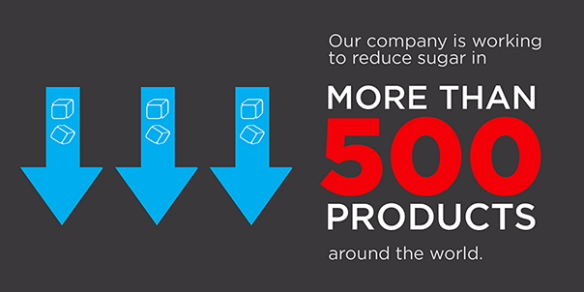
\includegraphics[width=0.9\textwidth]{assert/img7.png}
        \caption{Hình minh họa quảng cáo việc cắt giảm lượng đường của Coca-Cola}
        \caption*{(Nguồn: \href{https://www.coca-cola.com/pk/en/about-us/faq/how-does-the-company-address-obesity}{https://www.coca-cola.com/pk/en/about-us/faq/how-does-the-company-address-obesity})}
        \label{fig:img7}
    \end{figure}

    \vspace{0.2cm}
    Trên khắp các danh mục đầu tư, Công ty đang cắt giảm lượng đường trong danh  mục đồ uống hiện tại của mình bằng các công thức mới nhưng vẫn giữ được hương vị mà người tiêu dùng ưa chuộng, bên cạnh đó Công ty còn tung ra thương hiệu Coca-Cola Zero Sugar và các thương hiệu không đường/ít đường khác trên thị trường toàn cầu. Đồng thời công tác chuẩn bị phát triển các sản phẩm với bao bì kích cỡ nhỏ hơn như lon mini (lon nhỏ) đang là ưu tiên hàng đầu của công ty.

    \vspace{0.2cm}
    Ông Quincey: “Chúng tôi hiểu rằng để thúc đẩy sự phát triển bền vững và khả năng sinh lợi của thương hiệu thì cần phải khuyến khích và hỗ trợ người tiêu dùng kiểm soát được lượng đường dung nạp vào cơ thể. Chúng tôi luôn đề cao ý thức trong từng nỗ lực của mình để không chỉ mở rộng mà còn phải định hình danh mục đầu tư một cách trọn vẹn nhất”.

    \vspace{0.2cm}
    Quincey cho biết, công ty luôn ủng hộ khuyến cáo của Tổ chức Y tế Thế giới (WHO) và của nhiều cơ quan y tế khác trong việc duy trì lượng đường bổ sung thấp hơn 10\% lượng calo hấp thụ hàng ngày và nhận thấy cơ hội phát triển dựa trên các khuyến cáo này đang theo “cấp số lũy thừa”

    \vspace{0.2cm}
    $\Rightarrow$ Có thể thấy việc quan tâm và bảo vệ sức khoẻ của người tiêu dùng là một vấn đề  mà Coca Cola đang nỗ lực rất nhiều  để cải thiện trong từng sản phẩm. Điều này càng làm nổi bật biểu hiện trong việc thể hiện đạo đức kinh doanh của Công ty.

    \subsubsection{Đầu tư vào các loại nước giải khát mà người tiêu dùng mong muốn}
    \vspace{0.2cm}
    Coca-Cola sẽ mở rộng danh mục đầu tư của mình ở năm lĩnh vực, bao gồm: 
    \begin{itemize}
        \item Thức uống có ga,
        \item Thức uống bổ sung năng lượng,
        \item Sữa, nước trái cây có nguồn gốc từ thực vật,
        \item Thức uống dành cho việc thể thao và nước khoáng,
        \item Thức uống trà và cà phê pha chế sẵn.
    \end{itemize}

    \vspace{0.2cm}
    Coca Cola nhận định: “Trong quá khứ, lẽ ra chúng tôi phải dành nhiều thời gian hơn để tập trung vào các loại sẽ thịnh hành nhất sau này, thay vì theo xu hướng của phần lớn người tiêu dùng, và đó mới chính là giá trị lớn nhất của chúng tôi”

    \vspace{0.2cm}
    $\Rightarrow$ Mở rộng thị trường là điều cần thiết trong kinh doanh. Nhưng mở rộng thị trường mà vẫn đáp ứng được nhu cầu của người tiêu dùng mới là điều quan trọng hơn cả. Coca Cola luôn muốn đem lại cho người tiêu dùng những sản phẩm mang giá trị và chất lương nhất, thể hiện tận tâm từng khâu sản xuất kinh doanh.

    \subsubsection{Cạnh tranh song phẳng với các đối thủ trên thị trường}
    \vspace{0.2cm}
    Bất chấp những cạnh tranh khốc liệt trên thị trường, Coca-Cola vẫn giữ được tầm ảnh hưởng của một thương hiệu lớn, khi trải qua nhiều năm, vị thế của Coca-Cola trong lòng người tiêu dùng vẫn không thay đổi.
    \begin{itemize}
        \item \textbf{Liên tục tạo ra các thương hiệu mới để ngăn cản sự lấn át của đối thủ:}
        
        Theo một trong những marketer hàng đầu của Coca-Cola, trong bối cảnh mà số lượng các nhà bán lẻ trực tuyến như Amazon đang ngày càng gia tăng, việc cho ra đời những nhãn hiệu mới và gây dựng lòng trung thành giữa những người tiêu dùng là mấu chốt dẫn đến thành công. Nhận thức được sự bành trướng của các trang bán hàng trực tuyến, Javier Meza, CMO của Coca-Cola đã phát biểu tại buổi họp báo ở Atlanta, Mỹ: “Cách duy nhất để tồn tại trong kinh doanh là tạo ra những thương hiệu mới. Giây phút chúng ta ngừng việc tạo ra các nhãn hiệu cũng chính là lúc các nhà bán lẻ trực tuyến sẽ giành quyền thống trị.”
        \item \textbf{Luôn nhạy bén và chủ động trước những thay đổi của thị trường:}
        
        Đề cập đến chủ trương đổi mới của CEO James Quincey, người luôn tìm kiếm sự cải tiến trong các sản phẩm của Coca-Cola để đảm bảo doanh nghiệp sẽ luôn đón đầu các xu hướng mới trên thị trường cũng như nhu cầu thay đổi hàng ngày của người tiêu dùng, Meza chia sẻ: “Một khi tốc độ thay đổi ở bên ngoài công ty cao hơn bên trong, bạn sẽ phải nhận thất bại.” 

        Cũng theo lý giải của ông, lý do mà Coca-Cola có thể tạo ra những điều khác lạ đó là vì hãng luôn mang ý niệm sẵn sàng để thử những điều mới mẻ. Nếu thử nghiệm không mang lại thành công đi chăng nữa thì chí ít họ cũng đã hiểu nhiều hơn về thị trường thông qua nó.
    \end{itemize}

    \vspace{0.2cm}
    $\Rightarrow$ Coca-Cola đã thành công trong việc duy trì vị thế của mình trên thị trường nước giải khát toàn cầu. Họ đã xây dựng được một thương hiệu mạnh và có sức ảnh hưởng lớn đến người tiêu dùng. Họ đã thành công trong việc tạo ra một hình ảnh tích cực cho thương hiệu của mình thông qua các chiến dịch quảng cáo sáng tạo và ý nghĩa.

    \subsubsection{Đặt ra những mục tiêu phát triển bền vững phù hợp với nguyên tắc đạo đức kinh doanh}
    \vspace{0.2cm}
    Coca-Cola đã đặt ra những mục tiêu phát triển bền vững cho riêng mình, trong đó có những mục tiêu lớn như:
    \begin{itemize}
        \item Bảo vệ khí hậu : Giảm 25\% lượng carbon từ chương trình "the drink in your hand"  (so với mức cơ bản năm 2010)
        \item Đóng góp xã hội: Hàng năm đóng góp ít nhất 1\% thu nhập từ hoạt động của công ty (OI). (\%OI; Tổng \$ doanh thu từ hoạt động của công ty)
        \item Nhân quyền \& quyền lao động: Tối thiểu 98\% đối tác đóng chai độc lập và 95\% nhà cung cấp tuân thủ các Nguyên tắc Hướng dẫn Nhà cung cấp (SGP) của chúng tôi.
        \item Trách nhiệm quản lý nước: Hoàn trả cho cộng đồng và thiên nhiên lượng nước tương ứng với những gì chúng tôi sử dụng để sản xuất và hoàn thiện đồ uống; (tỷ lệ nước sử dụng để sản xuất đồ uống (dựa trên khối lượng bán ra hàng năm) được trả lại cho cộng đồng và thiên nhiên; số lít nước sử dụng để sản xuất đồ uống được làm đầy trở lại)
        \item Nông nghiệp: Tìm thêm những nguồn nguyên liệu nông nghiệp trọng điểm một cách bền vững hơn.
    \end{itemize}

    \vspace{0.2cm}
    $\Rightarrow$ Những mục tiêu này không chỉ giúp Coca-Cola phát triển bền vững mà còn thể hiện trách nhiệm xã hội của doanh nghiệp đối với cộng đồng và môi trường. Điều này cũng giúp Coca-Cola xây dựng được hình ảnh tích cực trong mắt người tiêu dùng và các nhà đầu tư.
    
    \subsubsection{Quan tâm đến việc cải thiện môi trường bằng cách tạo ra “một thế giới không rác thải”}
    \vspace{0.2cm}
    Việc quan tâm đến tình hình môi trường là điều mà nhiều công ty đang còn chưa làm được. Có rất nhiều Công ty vẫn xả rác thải trong quá trình sản xuất kinh doanh, hoặc chưa biết cách chưa xử lý kịp thời rác thải. Chính điều đó đã khiến cho môi trường phải những tác động tiêu cực, ảnh hưởng đến khí hậu toàn cầu, thế giới ngày càng trở nên ô nhiễm. 

    \vspace{0.2cm}
    Để cải thiện tình trạng này, Coca-Cola có một bước tiến đáng khen. ông James Quincey, Chủ tịch kiêm Giám đốc điều hành Công ty Coca-Cola cho biết: "Người tiêu dùng trên khắp thế giới đều có mối quan tâm lớn đến hành tinh của chúng ta. Họ mong muốn và hy vọng các công ty như chúng ta trở thành những người tiên phong trong việc hỗ trợ tạo ra một thế giới không rác thải".

    \vspace{0.2cm}
    Tầm nhìn về một 'Thế giới không rác thải', chúng tôi đang đầu tư cho hành tinh này và không ngừng cải tiến bao bì của mình để góp phần đưa vấn đề bao bì của thế giới trở thành vấn đề thuộc về quá khứ." Ông Quincey trong chuyến đi tham dự  để tham dự cuộc họp thường niên Diễn đàn Kinh tế Thế giới (WEF) tại Davos, Thụy Sĩ cho biết công ty sẽ tiếp tục tập trung phát triển bao bì có khả năng tái chế 100\% và giảm lượng nhựa sử dụng trong vỏ chai.

    \vspace{0.2cm}
    "Chúng tôi tin rằng mỗi bao bì - bất kể có nguồn gốc từ đâu - đều có giá trị và vòng đời vượt xa khả năng sử dụng ban đầu", Quincey nói thêm. "Thứ nào tái chế được thì hãy tái chế. Vì thế, chúng tôi mong muốn hỗ trợ để tất cả mọi người ở khắp mọi nơi hiểu được mình có thể đóng góp thế nào cho hành trình này.".

    \vspace{0.2cm}
    $\Rightarrow$ Coca-Cola đã thể hiện trách nhiệm xã hội của mình bằng cách quan tâm đến môi trường và tạo ra một thế giới không rác thải. Điều này không chỉ giúp Coca-Cola xây dựng được hình ảnh tích cực trong mắt người tiêu dùng mà còn góp phần bảo vệ môi trường và phát triển bền vững.

\subsection{Bài học rút ra đối với doanh nghiệp Coca-Cola}
    \subsubsection{Xây dựng thương hiệu cá nhân mạnh và độ nhận diện cao.}
    
    \vspace{0.2cm}
    Thương hiệu là một trong những yếu tố quan trọng nhất quyết định đến thành công hay thất bại của Coca Cola. Qua hơn 100 năm phát triển, hãng đồ uống ít khi thay đổi công thức của Coke, sản phẩm đầu tiên và nổi tiếng nhất của hãng. Hãng tập trung marketing cho sự kiên định của mình, ngày nay, hàng tỉ người trên thế giới không xa lạ gì với logo tròn trắng đỏ, với hình dạng chai nước hay lon nước. Năm 2024, thương hiệu Coke được định giá khoảng 100 tỉ đô, nằm trong top 15 thương hiệu giá trị nhất thế giới (Nguồn: \href{https://www.statista.com/statistics/326065/coca-cola-brand-value/}{https://www.statista.com/statistics/326065/coca-cola-brand-value/}).

    \subsubsection{Đa dạng hóa sản phẩm, thâu tóm và mở rộng thị trường.}

    \vspace{0.2cm}
    Ngoài Coke, Coca cola sở hữu nhiều thương hiệu đồ uống khác, với đa dạng sản phẩm: Dasani (nước đóng chai), Minute Maid (nước ép đóng chai), Costa Coffee. Sản phẩm của các thương hiệu con của tập đoàn xuất hiện tại tất cả các châu lục trên thế giới. Ngoài doanh thu trực tiếp từ các sản phẩm, Coca Cola còn kiếm lợi nhuận từ các hoạt động mở rộng (venture) và đầu tư. 

    \begin{figure}[H]
        \centering
        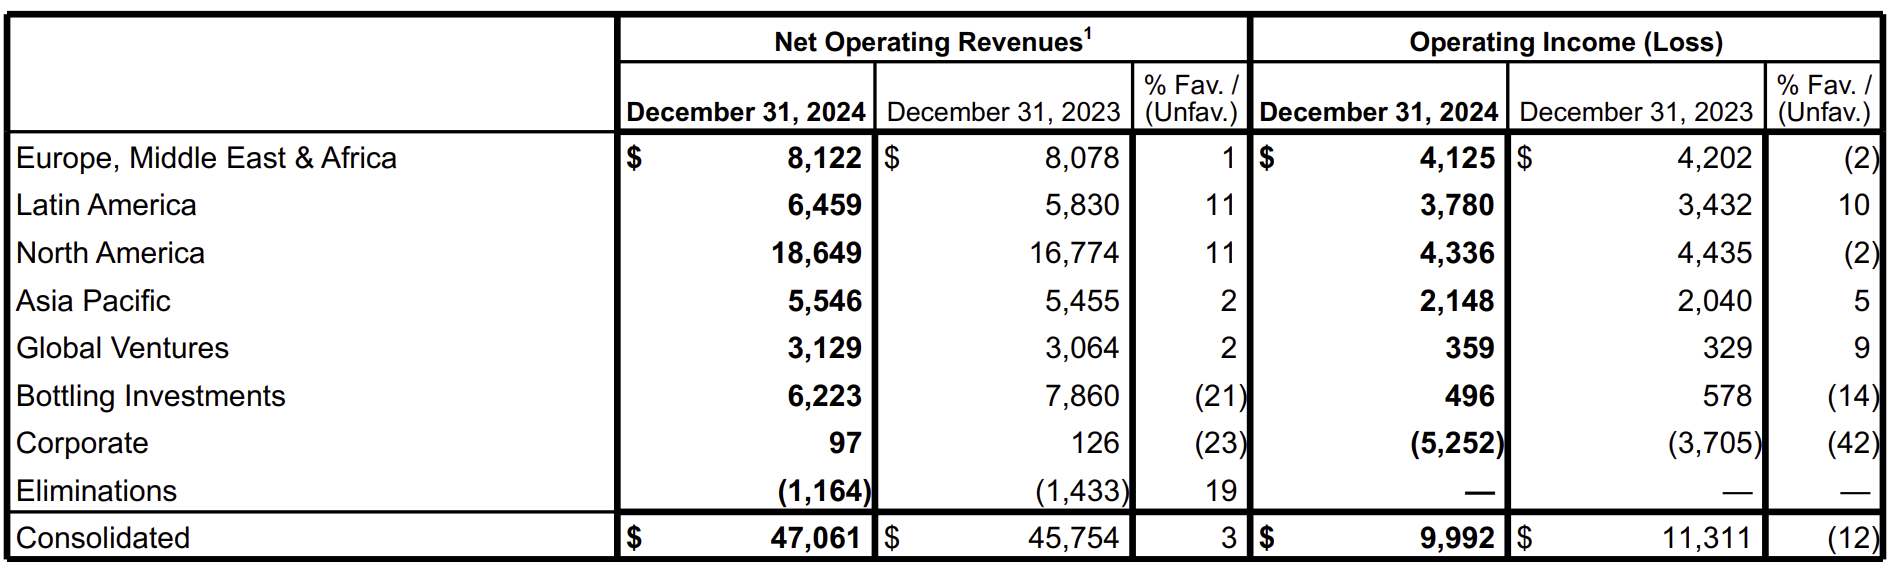
\includegraphics[width=0.9\textwidth]{assert/img8.png}
        \caption{Bảng doanh thu và lợi nhuận hoạt động theo khu vực của Coca-Cola trong năm 2024}
        \textit{(Đơn vị: triệu USD)}
        \label{fig:img8}
    \end{figure}

    \subsubsection{Cạnh tranh sòng phẳng và nhạy bén với các thay đổi của thị trường.}

    \vspace{0.2cm}
    Ngoài việc chủ động phát triển các sản phẩm mới và thâu tóm các thương hiệu con để cạnh tranh với các đối thủ đang lên, Coca Cola còn rất nhạy bén với các xu hướng về môi trường và đóng góp xã hội.
    \begin{itemize}
        \item Bảo vệ môi trường: Các sản phẩm của tập đoàn hướng tới mức độ tái chế cao, quá trình sản xuất được tối ưu hóa để giảm thiểu phát thải. Coca Cola hướng tới giảm 25\% lượng carbon phát thải. (Nguồn: \href{https://www.coca-cola.com/xe/en/sustainability/climate-action}{https://www.coca-cola.com/xe/en/sustainability/climate-action})
        \item Hằng năm đóng góp khoảng 1\% OI (Lợi nhuận lao động) cho xã hội thông qua việc đầu tư cho các ý tưởng kiến thiết hoặc giáo dục. (Nguồn: \href{https://www.coca-colacompany.com/social/coca-cola-foundation}{https://www.coca-colacompany.com/social/coca-cola-foundation})
        \item Đảm bảo nhân quyền và quyền lao động, 98\% đối tác đóng chai và 95\% nhà cung cấp của Coca Cola tuân thủ theo nguyên tắc nhà cung cấp (SGP) của tập đoàn.
        \item Hoàn trả cộng đồng và xây dựng nông nghiệp bền vững. Coca Cola đã đầu tư 1.5 triệu USD cho các dự án nông nghiệp bền vững tại Việt Nam, giúp cải thiện đời sống của 2000 hộ nông dân trồng mía đường.
    \end{itemize}

    \vspace{0.2cm}
    Những năm 2010s, Coca cola bán lại các cơ sở sản xuất và đóng chai cho các thương hiệu con và đối tác, bản thân Coca Cola tập trung hơn vào xây dựng thương hiệu, marketing và xây dựng chuỗi cung ứng. Coca Cola có một mối quan hệ nổi tiếng với đối thủ Pepsi. Suốt quá trình phát triển, có nhiều câu chuyện về việc hai thương hiệu tôn trọng công thức đồ uống của nhau. Trong các chiến dịch quảng bá sản phẩm của mình, cả hai cũng luôn rất sáng tạo và tôn trọng nhau, để đồng hành và cùng phát triển thay vì triệt hạ nhau.

    \vspace{0.2cm}
    $\Rightarrow$ Coca Cola có tầm nhìn về một thế giới không rác thải, họ luôn tìm cách cải thiện bao bì của mình. James Quincey - chủ tịch kiêm CEO của tập đoàn, trong chuyến tham dự cuộc họp thường niên Diễn đàn Kinh tế Thế giới (WEF) tại Davos, Thụy Sỹ cho biết công ty sẽ tiếp tục phát triển bao bì có khả năng tái chế 100\% và giảm thiểu lượng nhựa trong vỏ chai.


% ========================= Phần 3 ==========================
\newpage
\section{Kết luận và kiến nghị}
\subsection{Kết luận}
    \vspace{0.2cm}
    Đạo đức kinh doanh trong chiến lược marketing ở từng thời điểm phù hợp, Coca-Cola đã giữ được một chỗ đứng vững chắc trong lòng người tiêu dùng của Việt Nam nói riêng và thế giới nói chung. Nhờ những cố gắng không ngừng nghỉ để truyền tải những thông điệp nhân văn và thiết thực với nhiều người, Coca-Cola không còn là thức uống giải khát đơn thuần mà đã đi sâu vào tiềm thức như là một thương hiệu của sự lạc quan, không ngừng truyền cảm hứng và tạo ra những khoảnh khắc vui vẻ. 

\subsection{Kiến nghị}
    \subsubsection{Giải pháp trong hoạt động Marketing}
    \begin{itemize}
        \item Coca-Cola “chắc chân trên thị trường”, tập trung vào dòng sản phẩm chủ lực, tập trung vào các thị trường chủ chốt chứ không phải dàn trải để rồi không thu được gì trong cả năm.
        \item Công ty cần thực hiện các vụ thôn tính quan trọng trong khu vực đồ uống không có gas nhằm tăng cường sự hiện diện của mình tỏng phân khúc thị trường đang lên.
        \item Các chiến dịch Marketing cần phải bao quát rộng hơn những điểm liên quan đến người tiêu dùng như sử dụng những công nghệ tiếp thị mới từ hình thức quảng cáo 3D sang chương trình khác hàng lâu dài trực tuyến nhằm kết nối với người tiêu dùng, thu hút khác hàng tuổi teen – đây chính là đối tượng khách hàng có tiềm năng lớn để duy trì bền vững doanh thu của công ty.
        \item Tổ chức chiến dịch PR ở những trung tâm thương mại lớn như Tràng Tiền Plaza (Hà Nội), Metro (Đà Nẵng, Tp Hồ Chí Minh, …)
        \item Phát triển kênh phân phối: Coca-Cola phải tập trung vào xây dựng cho mình một hệ thống phân phối rộng rãi hơn nữa và đủ mạnh để lan tỏa sản phẩn của mình đến mọi tầng lớp người tiêu dung. Kết hợp cùng các dịch vụ, đội ngũ Marketing của Coca-Cola phải nhanh nhẹn hơn nữa để tìm ra những cơ hội mới. Trong thời kì hội nhập hiện nay, việc các dịc hvuj ăn uống mới từ nước ngoài chọn Việt Nam là “Địa điểm đóng đô” sẽ có xu hướng tăng thì Coca-Cola sẽ kết hợp với ác chuỗi của hàng, dịch vụ đó để bán sản phẩm của mình.
    \end{itemize}

    \subsubsection{Giải pháp trong hoạt động quản trị}
    \begin{itemize}
        \item Tiến hành “cú hích” Việt hóa nhân sự cấp cao nhằm thay đổi nhận thức của các công ty đa quốc gia về chất xám và tay nghề của lao động tại chỗ. Nên sử dụng nhiều lao động Việt Nam trong cơ cấu của công ty bời vì lao động Việt Nam cũng có trình độ không kém gì lao động các nước khác, hơn nữa, sử dụng lao động nội địa cũng là một lợi thế cho Coca-Cola trong công cuộc chinh phục người tiêu dung Việt Nam.
        \item Bản thân lãnh đạo cần là tấm gương về văn hóa doanh nghiệp
        \begin{itemize}
            \item \textbf{Về đối ngoại:} Nhà lãnh đạo cần xác định chiến lực hoạt động của công ty về thị trường.
            \item \textbf{Về đối nội:} Nhà lãnh đạo cần chịu trách nhiệm đề ra các quy định, lề lối làm việc nhằm khuyến khích sự sáng tạo trong việc của nhân viên.
        \end{itemize}
        \item Theo phong cách dân chủ, gần gũi với cấp dưới và nhân viên, các nhà lãnh đạo của công ty kiểm tra hình vi của cáp dưới để gia tăng việc thực hiện tốt công việc của họ theo những hình thức sau:
        \begin{itemize}
            \item Nếu nhân viên thực hiện có kết quả tốt, họ phải được thưởng để củng cố và duy trì hành vi, ngược lại nếu việc thực hiện của một nhân viên không có kết quả thì nhà quản trị xem xét xem nguyên nhân là gì? Nếu là do khả năng yếu kém thì nhà quản trị cần quyết định tổ chức một lớp huấn luyện cho nhân viên này.
            \item Nhà quản trị công ty không tuyển chọn nhân viên một cách bừa bãi.
            \item Nhà quản trị của công ty cần cung cấp cho hầu hết các nhân viên ột sự mô tả công việc của họ để làm rõ những nội dung gì bao gồm công việc của họ? Họ phải chịu trách nhiệm với ai? Những gì thuộc quyền của họ?
            \item Huấn luyện cho nhân viên công ty là nhằm tạo cho họ những hành vi và thái độ làm việc tốt hơn.
        \end{itemize}
    \end{itemize}

    \subsubsection{Giải pháp trong hoạt động sản xuất}
        \begin{itemize}
            \item Cần cải tiến công nghệ để đáp ứng nhu cầu của khách hang và cạnh tranh đối với các đối thủ trong và ngoài ngành.
            \item Cần có những thay đổi để đáp ứng đặc điểm và thị yếu của người tiêu dung.
            \item Hoạt động cần nhấn mạnh đến vấn đề an toàn chất lượng sản phẩm.
            \item Công ty cần tạo ra các sản phẩm thân thiện với môi trường, không gây ảnh hướng đến môi trường tự nhiên.
            \item Cần tái chế hiệu quả với vỏ lon nước ngọt.
            \item Cần tìm kiếm nguyên nguyễn liệu mới giúp vận hành hiệu quả, tiết kiệm chi phí sản xuất.
            \item Nâng cao sản xuất đảy mạnh các hoạt động truyền thống, quảng bá thương hiệu, đa dạng hóa sản phẩm nhằm thu hút khách hang trước sự đe dọa của các hãng khác.
            \item Đi theo hướng kinh doanh vền vững với những sáng kiến như tiết kiệm nước trong quá trình sản xuất, vật liệu khi đóng gói và thậm chí là cả điện năng của hang triệu tủ lạnh của các hang trên khắp các thế giới.
        \end{itemize}
\end{document}
